\documentclass{article}
\usepackage{tmlr}                % anonymous submission version  <-- ACTIVE
% \usepackage[accepted]{tmlr}    % camera-ready (authors visible)
% \usepackage[preprint]{tmlr}    % arXiv preprint

\usepackage{url}
\usepackage{booktabs}
\usepackage{amsmath,amssymb,amsthm}
\usepackage{graphicx}
\usepackage{multirow}
\usepackage{xcolor}
\usepackage{algorithm}
\usepackage{algpseudocode}
\usepackage{threeparttable}

\theoremstyle{plain}
\newtheorem{theorem}{Theorem}
\newtheorem{proposition}{Proposition}
\newtheorem{lemma}{Lemma}
\newtheorem{corollary}{Corollary}
\theoremstyle{definition}
\newtheorem{definition}{Definition}
\newtheorem{assumption}{Assumption}
\theoremstyle{remark}
\newtheorem{remark}{Remark}

\DeclareMathOperator*{\argmax}{arg\,max}
\newcommand{\Risk}{\mathcal{R}}
\newcommand{\Cov}{\mathcal{C}}
\newcommand{\emit}{\mathcal{E}}
\newcommand{\E}{\mathbb{E}}
\newcommand{\Iota}{\mathcal{I}}

\title{Certified Correction of Vision--Language Hallucinations:\\
Gains, Preconditions, and a Sequential Failure Mode}

% Camera-ready author block. Ignored while the anonymous \usepackage{tmlr} is active;
% restore [accepted] above to reveal it.
\author{%
  \name Quang-Vinh Dang \email vinh.dq4@buv.edu.vn \\
  \addr British University Vietnam, Hung Yen, Viet Nam
  \AND
  \name Phuong-Lan Nguyen \email 30066017@st.buv.edu.vn \\
  \addr British University Vietnam, Hung Yen, Viet Nam
}

\def\month{07}
\def\year{2026}
\def\openreview{\url{https://openreview.net/forum?id=ANONYMOUS}}

\begin{document}
\maketitle

\begin{abstract}
Selective prediction equips a vision--language model (VLM) with a distribution-free
guarantee on the answers it emits, and pays for that guarantee by abstaining on the rest.
A recent impossibility result shows the bill cannot be reduced by better engineering: when
the base risk $\mu$ exceeds the target $\alpha$, \emph{any} predictor that may only
\emph{emit or abstain the model's own answer} must abstain on at least
$(\mu-\alpha)/(1-\alpha)$ of inputs, whatever its score, bound, or calibration budget.
This paper takes that premise seriously and asks what changes when the predictor is
permitted to emit a \emph{different} answer. We introduce Certified-Correction Risk
Control (CCRC): accept the model's answer where a correctness score is high, substitute an
answer supplied by an \emph{independent} evidence channel where that channel's evidence is
strong, abstain otherwise, and certify the error rate of everything emitted at level
$\alpha$ with confidence $1-\delta$.

We prove validity for CCRC, characterise its behaviour, and evaluate it across five
benchmarks, two backbones and a mitigation decoder. Four findings organise the paper, and \S\ref{sec:intro} lists the five contributions they
support.
First, the correctness \emph{score} matters more than the procedure: a detection-grounded
score improves certified coverage over model-internal uncertainty by $11.9$--$32.1$ points,
and we decompose our total margin over a published CLIP-based scorer to show that $62.6$ of
$67$ points come from the score rather than from our algorithm. Second, repairs cannot be
self-certified --- we prove that certifying a substitution with the complement of the score
that flagged it is circular, and confirm that the resulting procedure repairs nothing.
Third, where CCRC helps it does so by \emph{dilution}: $0.9$--$1.8\%$ of items repaired at
a strict evidence gate buys $1.9$--$3.4\times$ that mass in certified coverage, because
high-precision repairs lower the emitted set's average risk and relax the binding
constraint; we give a diagnostic, checkable before calibration, that is consistent with both the
gains and the single dataset on which CCRC loses. Fourth, the natural generative extension
fails: in a paired matched-prefix experiment, repairing a claim mid-caption significantly
\emph{increases} downstream hallucination ($+0.207\pm0.091$ mentions, $n=121$, $p=0.025$),
which closes off a fixed-point calibration argument (correction-map monotonicity, not the
risk monotonicity in $\lambda$ that our one-shot guarantee avoids needing) and exposes an unpriced cost that a
context-blind sequential procedure must charge for. We also reproduce the closest concurrent method and
find the two mechanisms are complementary rather than competing. Code, extracted per-item
signals, and all negative results are released.
\end{abstract}

%===============================================================================
\section{Introduction}
\label{sec:intro}

\subsection{A small failure, and three unsatisfying options}

Image 518 of the POPE benchmark is an office desk. At its lower right, small but unoccluded and
plainly visible, is a computer mouse. We ask LLaVA-1.5-7B: \emph{``Is
there a mouse in the image?''} The model answers \textbf{no}, and it is not especially
confident about it --- the probability mass on \texttt{yes} is $0.207$. Our calibrated
correctness score for this item is $s=0.18$, at roughly the $0.2$nd percentile of the score distribution. An
open-vocabulary detector, asked independently whether it can localise ``a photo of a
mouse'' in the same pixels, returns a confidence of $0.903$ with a margin of $0.753$ over
its own negative-class baseline. The object is there. The detector sees it. The model
does not.

Now suppose we must ship this system with a promise: \emph{among the answers we actually
emit, at most $10\%$ are wrong, with $90\%$ confidence, and this must hold for the next
batch of inputs rather than the one we tuned on}. Such promises are what conformal risk
control was built to deliver, and the machinery is by now standard
\citep{vovk2005,bates2021rcps,angelopoulos2021ltt}. The standard recipe has exactly one
lever: a threshold on a correctness score, calibrated on held-out data, above which we
emit the model's answer and below which we abstain.

Applied to item 518, the recipe has three options, and all three are unsatisfying.

It can \textbf{emit} the answer. But $s=0.18$ is low, and if we set the threshold low
enough to admit this item we also admit a large population of items that genuinely are
uncertain and genuinely are wrong; the risk budget is consumed and the guarantee fails.

It can \textbf{abstain}. This is what every conformal method for vision--language models
we are aware of does, and it is safe. It is also, here, absurd: we are declining to answer
a question to which a component already inside our own system supplies the correct answer
with high confidence. We pay a coverage cost for an item we could have got right.

It can \textbf{delete the claim} --- the claim-filtering move used in the generative
setting \citep{conflvlm,conformalfactuality}. In a yes/no setting deletion is abstention.
In a captioning setting it is slightly better than abstention and considerably worse than
what a reader wants, since a caption with a hole in it is not a caption that has been
corrected.

What none of the three can do is emit \textbf{yes}. That option is not missing because it
was tried and found wanting. It is missing because the framework does not contain it. The
action space of a conformal selective predictor is $\{\text{emit the model's answer},
\text{abstain}\}$, and this paper is about what happens when a third action ---
\emph{emit a different answer, and certify that too} --- is added to it.

\subsection{Two literatures that do not meet}

The reason the fourth action is absent is, we think, sociological as much as technical:
the two research communities with a stake in it work on different halves of the problem
and rarely cite each other.

\paragraph{One literature makes the model wrong less often.}
This is by far the larger body of work, and it is inventive. It modifies decoding to
penalise the attention patterns associated with neglecting the image in favour of the
language prior
\citep{opera}; contrasts logits from clean and corrupted views of the image
\citep{vcd,degf}; localises the failure to particular layers and heads and intervenes
surgically \citep{attnlens,only,maskcd,causalgating}, or corrects the positional prior that
biases where the model looks \citep{mcallava}; injects the output of a
vision expert during generation \citep{marine}; verifies and rewrites after the fact
\citep{woodpecker,lure,reverse}; or grounds the model in retrieved external knowledge
\citep{mkgrag,rule}. The measured effects are substantial and the methods are cheap. But
the output of this literature is always of the form \emph{our hallucination rate is lower
than theirs on this benchmark}. A deployer who asks ``what fraction of the claims you emit
tomorrow will be false?'' gets an empirical average over a fixed test set, which is not an
answer to the question asked.

\paragraph{The other literature answers that question, and charges for it.}
Conformal prediction and its risk-control descendants turn any heuristic score into a
decision rule with a finite-sample, distribution-free guarantee. Applied to generation,
the result is \emph{selective prediction}: emit when a correctness score clears a
calibrated threshold, abstain otherwise, and the error rate \emph{among emitted outputs}
is at most $\alpha$ with probability $1-\delta$
\citep{conformallm,conformalfactuality,conflvlm,onlineabstention}. This is exactly the
promise a deployer wants, it holds without distributional assumptions beyond
exchangeability, and it holds for the next batch and not merely the last one. The price is
paid in coverage: every item the rule cannot vouch for is an item nobody is served.

Neither literature is wrong. But notice what falls between them. The first literature
builds systems that can \emph{repair} a wrong answer --- Woodpecker rewrites captions with
detector output, REVERSE resamples flagged spans, MARINE injects object-level guidance ---
and never certifies the result. The second literature certifies rigorously and never
repairs. The obvious composition, \emph{certified repair}, is what the verify-and-correct line
\citep{woodpecker,lure,cmvkgguard} gestures at without achieving: pipelines whose
correctness rests on benchmark averages. This paper asks the question that line leaves
open --- what would it take to attach a real guarantee to a system that changes its own
answers?

\subsection{The price of a guarantee, and why it is not a tuning problem}

Before asking that, it is worth being precise about how expensive abstention is, because
the size of the number is what makes the fourth action interesting rather than merely
tidy.

\citet{crcimposs} give the answer in closed form. If the base risk of the underlying model
is $\mu$ and the target is $\alpha<\mu$, then \emph{any} conformal selective predictor must
abstain on at least
\[
  \frac{\mu-\alpha}{1-\alpha}
\]
of inputs. The bound does not depend on the quality of the score, the
tightness of the concentration inequality, or the size of the calibration set. A perfect
oracle score obeys it. A larger calibration set does not relax it. It is a property of the
action space, not of the estimator.

The consequences on real systems are not subtle. On our POPE-1500 setup with LLaVA-1.5-7B
the empirical base risk is $\mu\approx0.18$; at $\alpha=0.10$ at least $8.9\%$ of inputs
must be refused before any method is chosen. Our own tuned filtering pipeline, which is
competitive with published conformal VLM results, certifies $42.1\%$ coverage on
POPE-adversarial at $\alpha=0.10$: three in five questions go unanswered. On
HallusionBench, where the base risk is high enough that the floor swallows the entire
budget, it certifies $0.0\%$. Zero. The guarantee holds vacuously, over an empty emitted
set, which is exactly the failure mode a practitioner would call useless.

This is the point at which the natural engineering instinct --- \emph{find a better score}
--- runs into the theorem. A better score moves you toward the floor faster. It cannot move
you through it. Whatever is to be done must be done to the action space.

\subsection{Re-reading the premise}

So we re-read the premise. \citet{crcimposs} state it plainly: the predictor may only emit
the model's own answer or abstain. Every conformal method for VLMs we surveyed satisfies
it, and satisfies it structurally rather than incidentally. Claim-filtering deletes
unsupported claims \citep{conflvlm,conformalfactuality}. Abstention methods decline
\citep{onlineabstention,twoaxes}. The closest concurrent work, budgeted conformal evidence
acquisition \citep{bcea}, acquires \emph{additional visual evidence} for borderline claims
and re-scores the original assertion --- a genuinely clever move that buys real coverage,
and one that explicitly leaves the emitted answer unchanged. In every case the object
emitted is the model's output or nothing.

Item 518 says that this is a choice, not a necessity. Our system already contains a
component that knows the right answer. The question is whether we can emit that answer
\emph{and still have a guarantee}.

\paragraph{What changes.}
Permitting substitution does not evade the mathematics; it changes the object being
certified. If the emitted answer may originate outside the model, the quantity to control
is the risk of a \emph{mixture} --- accepted model answers together with substituted ones
--- and the bound of \citet{crcimposs} no longer binds, because its premise is violated.
The guarantee must be re-derived for the mixture, which we do
(Theorem~\ref{thm:validity}), and the substitutions must come from somewhere trustworthy,
which turns out to be a hard constraint rather than an implementation detail
(\S\ref{sec:independence}).

\paragraph{Why it can win, in one sentence.}
High-precision repairs are \emph{low-risk} emissions. Adding them to the emitted set pulls
its average risk below $\alpha$, which slackens the binding constraint, which lets the
acceptance threshold move down, which admits a much larger population of ordinary
accepted items. The gain is therefore levered: in our experiments $0.9$--$1.8\%$ of items
repaired buys $1.9$--$4.7$ percentage points of certified coverage, a
$1.9$--$3.4\times$ multiplier. The mechanism is not ``we fixed some answers''; it is ``fixing a few answers
changed the price of all the others''.

\subsection{What went wrong on the way, and what it taught us}

It would be convenient to report that the idea worked. It works in four settings out of
five, and the interesting content of this paper is largely in the failures, each of which
turned out to be forced rather than accidental. We list them here because they are the
spine of the argument, and each is a section below.

\paragraph{The cheap version defeats itself.}
The first design certified repairs using the complement of the score that flagged the
original: if $s$ is low, surely $1-s$ vouches for flipping the answer. This is circular,
and we can say exactly how. For binary decisions the risk of the flipped answer on a
flagged region equals the model's \emph{accuracy} on that region, so a self-repair region
is cheap only where the model is right less than $\alpha$ of the time --- a strictly
stronger demand than finding a region where it is unconfident. We first thought this
impossible and can now be more precise: it is admissible whenever the accepted region has
slack (Proposition~\ref{prop:selfrepair}), but on the settings where correction is worth
doing the region does not exist ($20.9\%$ accuracy in the bottom $2\%$ of our score against
$\alpha=0.10$; $64.3\%$ on Qwen2-VL), and attempting it makes the fixed sequence abort
outright on $65$--$100\%$ of splits. So a second, independent channel is required in
practice, which is the paper's main structural claim --- an empirical regularity with a
mechanism, not a theorem.

\paragraph{The obvious parameterisation loses on half our backbones.}
Given two channels, the natural move is to sweep both gates with the single risk-control
parameter. We did, and it lost $4.2$ points on Qwen2-VL and $2.9$ on VCD-decoded LLaVA
relative to plain filtering, because a liberal acceptance threshold drags the repair gate
open with it and admits low-precision repairs precisely when the budget is tightest. The
fix is to decouple: the repair gate is fixed and strict, and only acceptance is calibrated
(\S\ref{sec:decoupling}). This is a small change with a large effect, and we report the
version that failed because the reason it failed is the reason the final design looks the
way it does.

\paragraph{The gains are real, modest, and not uniform.}
Averaged over settings the improvement is a few points of certified coverage, with one
reversal. We chased the reversal and found a partial explanation: the achievable gain is
capped by the abstained mass, so a benchmark that already certifies most of its inputs has
little to gain and the same exposure to loss. This yields a checkable diagnostic --- $\mu$
comfortably above $\alpha$, with an applicable evidence channel --- which is consistent
with the failure on AMBER-discriminative but, being an upper bound on the gain, does not
predict it (\S\ref{sec:precondition}, Remark~\ref{rem:notprediction}). Upside is bounded;
downside is not.

\paragraph{Most of our headline margin is not our algorithm.}
Compared against a published conformal VLM scorer we gain about $67$ points of certified
coverage on one setting. Decomposed, roughly $62.6$ of those points come from the
correctness score --- a boring combination of logit and grounding features --- and
around $4.4$ from the certified-correction mechanism itself. We report the decomposition
rather than the headline (\S\ref{sec:attribution}), and we would rather a reader trust the
$4.4$ than be sold the $67$.

\paragraph{In generation, correction backfires.}
The motivating case for repair is generative: replacing a hallucinated object word is
plainly more useful than deleting the sentence containing it. Extending the guarantee to a
sequence requires that repairing a claim not make later claims worse --- a monotonicity
property that would license a fixed-point argument. We tested it directly with a paired
matched-prefix design and it fails: repaired prefixes yield $+0.207\pm0.091$ additional
hallucinated mentions downstream ($n=121$, $p=0.025$). The fixed-point route --- which needs the correction map to be monotone --- is closed. We
give the weaker coupling bound that survives (Theorem~\ref{thm:coupling}) and report the
failure as a finding, since it constrains anyone attempting on-policy certified editing.

\paragraph{The closest competitor turns out to be an ally.}
Concurrent work \citep{bcea} shares our benchmarks, our machinery, and our motivation, and
we initially read it as a scoop. Reproducing it under a common base score shows the two
mechanisms rescue disjoint populations of claims --- theirs the ones where more looking
resolves the doubt, ours the ones where the model is simply wrong and something else is
right --- and compose additively (\S\ref{sec:bcea}). We narrow our novelty claim
accordingly, to the substitution action and its guarantee.

\medskip
We report all of this. The paper is arranged so that each design decision is forced by a
measurement rather than asserted, and the negative results appear as findings rather than
as caveats appended to a positive headline.

\subsection{Contributions}
\begin{enumerate}
\item \textbf{A procedure and its guarantee} (\S\ref{sec:method}). CCRC emits accepted,
repaired, or abstained outputs and certifies the risk of the emitted mixture:
$\Pr[\Risk(\emit)\le\alpha]\ge1-\delta$ (Theorem~\ref{thm:validity}), using
fixed-sequence testing over a nested policy family with exact binomial bounds. We also
give the minimum certifiable sample size (Lemma~\ref{lem:kmin}), a small result with
practical teeth: a fixed sequence started below it aborts and returns zero coverage.

\item \textbf{Why repair cannot be self-certified in practice}
(\S\ref{sec:independence}). Certifying a substitution using the complement of the score
that flagged the original makes the repair's risk equal to the model's \emph{accuracy} on
the flagged region. Proposition~\ref{prop:selfrepair} bounds the mass such a repair may
occupy by the accepted region's slack; we then measure that on the settings where
correction is worth doing no sufficiently low-accuracy region exists, and that the
fixed-sequence test aborts entirely on $65$--$100\%$ of splits when self-repair is
attempted. The conclusion --- use a second, independent channel --- is an empirical
regularity with a mechanism, not a theorem.

\item \textbf{A mechanism and a precondition} (\S\ref{sec:mechanism},
\S\ref{sec:precondition}). We show why repair helps when it helps: high-precision repairs
lower the emitted set's average risk, relaxing the binding constraint and permitting a more
permissive acceptance threshold (Proposition~\ref{prop:dilution}). The effect is levered:
$0.9$--$1.8\%$ repaired mass yields $1.9$--$4.7$ points of coverage. We then bound the
achievable gain by the abstained mass (Proposition~\ref{prop:precondition}), which
explains the asymmetry we observe --- upside is capped, downside is not --- and yields a
diagnostic that is consistent with, though it does not predict, the one benchmark where
CCRC loses.

\item \textbf{A sequential negative result} (\S\ref{sec:sequential}). In a paired
matched-prefix experiment on free-form captions, repairing a hallucinated claim
significantly increases hallucination in the continuation. This rules out the \emph{correction-map} monotonicity on which a fixed-point argument for an
on-policy sequential guarantee would rest (a different property from risk monotonicity in
$\lambda$, which Theorem~\ref{thm:validity} never uses), and we give the
weaker coupling bound that survives (Theorem~\ref{thm:coupling}).

\item \textbf{Honest attribution and positioning} (\S\ref{sec:attribution}). We decompose
our margin over a published scorer and report that most of it is the score, not the
procedure. We reproduce the closest concurrent method \citep{bcea} and find the two
mechanisms compose rather than compete.
\end{enumerate}

\subsection{Roadmap}
\S\ref{sec:related} situates the work between the two literatures above.
\S\ref{sec:setup} fixes notation and derives the abstention floor in our own terms, so
that the object CCRC certifies can be compared with it directly. \S\ref{sec:method} gives
the procedure, its guarantee, the impossibility result, the decoupling argument, the
dilution mechanism, and the precondition. \S\ref{sec:exp} reports experiments across five
benchmarks, two backbones and one mitigation decoder, including the setting where the
method fails and the baselines that narrow the credit due to it. \S\ref{sec:sequential}
reports the sequential falsification and what survives it. \S\ref{sec:ablations} isolates
the score combiner (with a validity trap we fell into), the choice of concentration bound,
and positioning against prior art. \S\ref{sec:discussion} states the limitations we
consider load-bearing.

%===============================================================================
\section{Related work}
\label{sec:related}

This section is organised around the gap identified in \S\ref{sec:intro}. We first survey
what is known about hallucination in vision--language models and the very large body of
work that reduces it (\S\ref{sec:rel:hallu}), noting throughout that essentially none of it
produces a guarantee. We then survey distribution-free risk control
(\S\ref{sec:rel:conformal}) and its application to language and vision--language generation
(\S\ref{sec:rel:conflm}), noting that essentially all of it operates by deletion or
abstention. \S\ref{sec:rel:uq} covers non-conformal uncertainty quantification, which
supplies many of the scores both literatures use. \S\ref{sec:rel:position} treats the two
concurrent papers that bear most directly on our claim, and \S\ref{sec:rel:shift}
the shift induced by acting on one's own output. \S\ref{sec:rel:summary} states what,
after all of this, we take to be new.

\subsection{Hallucination in vision--language models}
\label{sec:rel:hallu}

\paragraph{Phenomenon, taxonomy and causes.}
Hallucination in multimodal models is conventionally decomposed by what is fabricated:
\emph{existence} (an absent object is asserted), \emph{attribute} (a present object is
described wrongly), and \emph{relation} (spatial or interactional claims that do not hold)
\citep{amber}. Surveys of the multimodal case \citep{bai2024survey,liu2024survey} and of
the text-only antecedent \citep{ji2023} converge on a small set of proximate causes. First,
\emph{language-prior dominance}: the autoregressive decoder is trained on text in which
certain objects co-occur, and at generation time it will complete ``a desk with a keyboard
and a\dots'' with \texttt{mouse} whether or not a mouse is visible. Second, \emph{visual
under-attention}: attention mass on image tokens decays with position, so later tokens in
a long caption are generated with progressively less visual grounding. Third,
\emph{instruction-tuning artefacts}: supervision built from captions that describe more
than is visible teaches the model to over-describe \citep{liu2023lrv}. Fourth, ordinary
\emph{miscalibration} of the underlying classifier \citep{guo2017}, which matters for us
because it determines how informative the model's own logits are as a correctness score.

The taxonomy is not decoration; it determines which evidence can refute a claim, and
therefore which claims a system like ours can repair. Existence claims are checkable by an
open-vocabulary detector \citep{owlv2,liu2024groundingdino}. Attribute claims require finer
perception than a detector supplies. Relation claims require structure that neither a
detector nor a similarity model represents. We return to this in \S\ref{sec:exp:noapply},
where the composition of a benchmark --- not its difficulty --- decides whether our
evidence channel applies at all.

\paragraph{Benchmarks, and what they measure.}
POPE \citep{pope} probes existence with balanced yes/no questions under three negative
samplings: \emph{random} objects, \emph{popular} (frequent in the corpus), and
\emph{adversarial} (frequently co-occurring with objects that are present). The last is
substantially harder precisely because it pits the language prior against the image, which
makes it the most informative split for our purposes. CHAIR \citep{chair} scores free-form
captions by the fraction of mentioned objects absent from MS-COCO ground truth, and remains
the standard generative metric despite its restriction to a closed vocabulary. AMBER
\citep{amber} provides an LLM-free benchmark with per-image lists of present and
hallucinated objects across generative and discriminative splits, and annotates attribute
and relation types as well as existence. MMHal-Bench --- introduced by \citet{sun2024aligning} alongside Fact-RLHF --- evaluates
diverse hallucination types in question answering using a strong judge model. MME \citep{mme}
measures broad perception and cognition across fourteen subtasks, only some of which are
grounding-checkable. HallusionBench \citep{hallusionbench} targets visual illusions,
charts, and reasoning traps, and is hard enough that strong models approach chance --- a
property that turns out to matter a great deal for any method with an abstention floor.
GQA \citep{gqa} supplies compositional questions over scene graphs.

We use POPE, AMBER, MME, GQA and HallusionBench. One methodological remark belongs here
rather than in the experiments: single-type AMBER subsets are label-degenerate (the
\texttt{hallucination} subset has all-\texttt{no} gold answers, the \texttt{relation}
subset all-\texttt{yes}), which inflates AUROC to $1.0$ for any score correlated with the
question type. We report on the mixed subset for this reason, and flag it because the
degeneracy is easy to miss.

\paragraph{Mitigation by decoding.}
The largest and most active family modifies the decoding distribution at inference time,
with no retraining. OPERA \citep{opera} identifies a columnar attention pattern over a few
\emph{summary} tokens, at which knowledge aggregates and image tokens are neglected,
penalises it in the beam score, and rolls back to re-allocate \emph{token selection} when
the pattern is detected. Visual contrastive decoding \citep{vcd} contrasts
logits computed from the clean image against logits from a diffusion-corrupted version,
subtracting the component of the distribution that survives visual degradation --- i.e.\ the
component driven by the prior. Other variants change what is contrasted: HALC \citep{chen2024halc} contrasts
adaptively selected fine-grained fields of view rather than a globally corrupted image, and
\citet{favero2024} formalise the contrast as an information-grounding objective. DeGF \citep{degf} closes a generative loop:
it synthesises an image from the candidate caption and diffs it against the input. MARINE
\citep{marine} injects object-level guidance from an external vision expert into the
decoding step, which is the closest decoding-time analogue of our evidence channel --- with
the difference that it steers the model rather than replacing its answer, and offers no
bound.

These methods are cheap, training-free, and demonstrably effective. Their relation to our
work is compositional rather than competitive: they lower the base risk $\mu$, while we
control the risk of what is emitted. Because the abstention floor is
$(\mu-\alpha)/(1-\alpha)$, \emph{any} reduction in $\mu$ directly relaxes the constraint we
operate under, so the two lines of work multiply rather than substitute. We verify this
empirically by running our layer on top of \citet{vcd} in \S\ref{sec:vcd}, and find both
that the composition works and that the coupled variant of our own method fails there ---
which is how we discovered the need to decouple the repair gate.

\paragraph{Mitigation by attention-level and mechanistic intervention.}
A related line localises hallucination to specific components and intervenes there.
Attention-lens style analyses trace hallucinated tokens to identifiable heads and layers
\citep{attnlens,only}, and interventions range from masking image heads
\citep{maskcd} to causal gating of the information paths implicated \citep{causalgating}. A
distinct line attacks the positional prior instead: MCA-LLaVA \citep{mcallava} replaces
RoPE's one-dimensional long-term decay with a two-dimensional Manhattan-distance spatial
decay, removing the bias that makes instruction tokens over-attend to bottom-right image
tokens. These give the most detailed available picture of
\emph{where} the failure lives. They are orthogonal to our concern, which is not where the
error comes from but what the emitted set's risk is once it exists; we cite them because
they are the strongest current evidence that hallucination is a structured, localisable
phenomenon rather than noise --- which is in turn why an independent channel can be
expected to be informative about it.

\paragraph{Mitigation by training and preference optimisation.}
A second family changes the model. Factually augmented RLHF \citep{sun2024aligning} scores
responses against ground-truth image content during reward modelling. RLHF-V
\citep{yu2024rlhfv} collects fine-grained \emph{correctional} human feedback --- humans
edit hallucinated segments --- and aligns on the edits, which is conceptually the closest
training-time analogue of certified correction, minus the certificate. Robust instruction
tuning \citep{liu2023lrv} attacks the artefact at its source by constructing negative
instructions. These require training and produce a better $\mu$; again, complementary.

\paragraph{Mitigation by post-hoc verification and rewriting.}
The third family is the one our work descends from: generate, then check, then change.
Woodpecker \citep{woodpecker} extracts object claims from a caption, queries detectors,
and rewrites the caption using a language model. LURE \citep{lure} identifies
hallucination-prone captions from co-occurrence and uncertainty statistics and revises
them. REVERSE \citep{reverse} trains the model to emit explicit confidence markers during
generation and then retrospectively resamples the spans it flagged, which makes it the
closest work in \emph{spirit} to ours: it also changes the output rather than deleting it.
Knowledge-grounded variants replace detectors with retrieval over multimodal knowledge
graphs \citep{mkgrag} or domain corpora \citep{rule}.

Every method in this family performs the same three steps we do --- flag, consult external
evidence, substitute --- and none of them certifies the substitution. The quantity they
report is a benchmark average after rewriting. \citet{cmvkgguard} is of exactly this type,
and the present paper can be read as asking what it would take to attach a guarantee to
such a pipeline. The attachment is not a matter of wrapping the pipeline in a
calibration loop: the natural way to certify a correction is circular
(\S\ref{sec:independence}), and the honest version requires an architectural
commitment that the verify-and-rewrite literature happens to satisfy by accident rather
than by design.

\subsection{Conformal prediction and distribution-free risk control}
\label{sec:rel:conformal}

\paragraph{From coverage to risk.}
Conformal prediction \citep{vovk2005,papadopoulos2002,lei2018} converts any score into
prediction sets with finite-sample marginal coverage under exchangeability alone; see
\citet{angelopoulos2023gentle} for a modern treatment. Refinements adapt the sets to local
difficulty \citep{romano2019}, exploit leave-one-out structure \citep{barber2021}, control
error per class \citep{sadinle2019,ding2023}, condition on groups
\citep{vovk2003mondrian}, and relax exchangeability itself \citep{barber2023}.

For our purposes the relevant generalisation is from \emph{coverage} to \emph{risk}.
Risk-controlling prediction sets \citep{bates2021rcps} bound the expectation of a monotone
loss rather than a miscoverage indicator. Conformal risk control
\citep{angelopoulos2024crc} extends this to a general family of monotone risks with a
single scalar parameter. Learn-Then-Test \citep{angelopoulos2021ltt} drops monotonicity
altogether and treats the choice of configuration as a multiple-testing problem, which is
the tool we need: our policy family is indexed by a threshold whose induced risk is
\emph{not} guaranteed monotone once repairs enter the emitted set, and LTT's
fixed-sequence testing lets us search a nested family at full $\delta$ without a
Bonferroni penalty.

\paragraph{The bound matters.}
Which concentration inequality supplies the per-hypothesis $p$-value has a large practical
effect at the sample sizes available in VLM calibration. Hoeffding's inequality is loosest;
empirical Bernstein adapts to observed variance; betting-style e-value constructions are
tighter again \citep{waudbysmith2024}. For a binary loss --- our case, since an answer is
right or wrong --- the exact Clopper--Pearson interval \citep{clopper1934} dominates all of
these, and we confirm the ordering experimentally in \S\ref{sec:ablations}. Anytime-valid
inference via e-processes and Ville's inequality \citep{waudbysmith2024,ramdas2023} extends
validity to data-dependent stopping, which is the natural machinery for sequence-level
guarantees and which we take up --- and find insufficient on its own --- in
\S\ref{sec:sequential}.

\paragraph{Selective prediction is older than conformal prediction.}
The accept/abstain trade-off dates to \citet{chow1970}; its statistical theory
\citep{elyaniv2010,bartlett2008,cortes2016} and its deep-learning instantiations
\citep{geifman2019} predate the conformal treatment. What conformal methods add is not the
idea of abstaining but the distribution-free, finite-sample character of the promise. It is
worth keeping the distinction in view, because the impossibility bound we build on is a
statement about the selective-prediction \emph{action space}, and therefore applies to the
classical formulations just as much as to the conformal ones. Learning-with-rejection
theory has, to our knowledge, likewise never considered a \emph{reject-and-substitute}
action with a risk certificate.

\subsection{Conformal methods for language and vision--language models}
\label{sec:rel:conflm}

\paragraph{Text.}
Conformal language modeling \citep{conformallm} calibrates sampling, stopping and
rejection rules so that the returned set of generations contains an acceptable output with
high probability. Conformal factuality \citep{conformalfactuality} decomposes an output
into sub-claims and \emph{backs off} --- progressively removing the least supported claims
--- until a factuality guarantee holds, which makes the emitted object a subset of the
original. Conformal alignment \citep{gui2024conformal} certifies which foundation-model
outputs are trustworthy enough to use. Multiple-choice settings admit a direct application
of split conformal prediction \citep{kumar2023}, and conformal machinery has been used to
calibrate when an LLM planner should ask a human for help \citep{ren2023knowno} --- an
action space of $\{$act, defer$\}$, again without substitution. Token-level and next-token
variants calibrate on entropy or logit statistics \citep{tecp,cover}. Online and
bootstrapped variants address feedback loops and estimator variance
\citep{onlineabstention,tamingvar}, and pipeline-level joint coverage over multiple stages
has been studied \citep{pasc}.

\paragraph{Vision--language.}
ConfLVLM \citep{conflvlm} is the closest published system in the multimodal setting. It
treats each generated detail as a hypothesis, scores it with a domain-appropriate heuristic
--- CLIP similarity \citep{clip} for natural-scene descriptions, BiomedCLIP for radiology,
LayoutLMv3 for documents --- and filters unsupported details, reporting a reduction in
claim error from $87.8\%$ to $10.0\%$ for LLaVA-1.5 scene descriptions at a stated
coverage cost. \citet{twoaxes} decompose the reliability question along a coverage axis and
a risk axis and study the trade-off directly.

\paragraph{The common operation.}
Across this entire body of work --- text and multimodal, offline and online, claim-level
and sequence-level --- the operation performed on a flagged claim is the same:
\textbf{deletion, abstention, or back-off}. This is the empirical basis for our reading of
\citet{crcimposs}: the premise of the impossibility bound is not an artefact of that
paper's formalism, it is a faithful description of what every method in the area actually
does. Nothing in the literature emits a claim the model did not produce and then certifies
the result.

\subsection{Uncertainty quantification without a guarantee}
\label{sec:rel:uq}

Our channel-1 score is not novel and we do not claim it is; it belongs to a large
literature on estimating generative uncertainty, which supplies the raw material that
conformal wrappers calibrate. Sequence likelihood and length-normalised logprobs are the
baseline. \citet{kadavath2022} show that models can be prompted to predict their own
correctness. Semantic uncertainty \citep{kuhn2023} clusters samples by entailment before
computing entropy, so that paraphrases do not count as disagreement, and semantic entropy
scales this into a practical hallucination detector \citep{farquhar2024}. Verbalised
confidence \citep{lin2022} elicits a probability in words. SelfCheckGPT \citep{manakul2023}
detects hallucination by sampling several generations and measuring mutual consistency,
which requires no logit access; self-consistency \citep{wang2023selfconsistency} uses the
same signal to improve accuracy rather than to flag. Calibration of the underlying
classifier \citep{guo2017} determines how much any of these are worth.

Two observations relevant to our design. First, all of these are \emph{self-referential}:
they interrogate the model about its own output. This is exactly the property that
\S\ref{sec:independence} shows to be fatal for certifying a correction --- a score
derived from the model cannot vouch for an answer that contradicts the model. Second, the
detectors used in the mitigation literature (open-vocabulary detection
\citep{owlv2,liu2024groundingdino}, image--text similarity \citep{clip}) are not
uncertainty estimates at all but independent perceptual evidence, and it is precisely their
independence, not their accuracy, that makes them usable as channel~2.

\subsection{The two closest works, and what separates us from them}
\label{sec:rel:position}

\paragraph{The impossibility bound.}
\citet{crcimposs} asks when conformal risk control can certify structured LLM outputs at
all, and the paper is best read as three results with one practical moral. First, the
impossibility result: when the base risk exceeds the target, any distribution-free method
must abstain on at least $(\mu-\alpha)/(1-\alpha)$ of examples. Because $\mu$ and $\alpha$
are both known before calibration, this doubles as a \emph{closed-form feasibility test} ---
one can determine whether CRC will work at all without running it. Second, a certification
hierarchy across Hoeffding, empirical Bernstein, and a betting-based e-CRC bound, with the
Hoeffding-to-Bernstein step supplying the largest single gain ($+37\%$ certified
configurations) and e-CRC earning its keep only when calibration data is scarce ($10\%$
certification at $20\%$ of the data against $0\%$ for Hoeffding). Third, a validation of
adaptive conformal inference under cross-dataset shift, cutting risk-target violations from
$71\%$ to $21\%$, with the residual failures concentrated exactly where the impossibility
bound predicts they must be. The empirical scope is substantial --- six open-weight models
from 3B to 72B parameters, eight datasets, four tasks, six nonconformity scores --- and its
verdict is blunt: hard NER, QA and classification configurations are simply uncertifiable
at $\alpha=0.10$.

Two things about this paper matter for us. The first is what it does \emph{not} study: the
setting is text-only structured generation (named-entity recognition, JSON extraction,
question answering, classification), so the multimodal case, where an independent
perceptual channel is available in a way it is not for pure text, is outside its scope. The
second is the remedy it recommends. Faced with infeasibility at $\alpha=0.10$, the
prescription is to \emph{relax the target}: at $\alpha=0.30$--$0.40$ certification becomes
practical ($47\%$ of NER, $40\%$ of QA, $60\%$ of classification configurations). That is a
sound recommendation and, for many deployments, the right one. It is also an admission
about the shape of the problem, and it is the fork this paper takes differently. We do not
weaken or contradict the bound --- it is correct, and we re-derive it in our own notation in
Proposition~\ref{prop:floor}. We exit its premise, and then pay for the exit by re-deriving
validity for the mixture (Theorem~\ref{thm:validity}) and by discovering the constraints
that substitution imposes (\S\ref{sec:independence} and Theorem~\ref{thm:coupling}). The
same author's pipeline-level conformal work \citep{pasc} composes stage-wise guarantees and
is subject to the same premise at every stage.

\paragraph{Three responses to one bound.}
It is worth naming the alternatives explicitly, because the contribution of this paper is
best understood as a choice among them. Given a base risk $\mu$ above the target $\alpha$,
the floor $(\mu-\alpha)/(1-\alpha)$ can be answered in exactly three ways.
\textbf{(i)~Relax the target.} Accept a weaker promise until it becomes feasible; this is
the recommendation of \citet{crcimposs}, and at $\alpha=0.30$--$0.40$ it works.
\textbf{(ii)~Lower $\mu$, or sharpen the score.} Every mitigation method in
\S\ref{sec:rel:hallu} does the former; \citet{bcea} does the latter, by spending a budget
to look again before deciding. Both stay inside the premise and both shrink the floor
without removing it. \textbf{(iii)~Change the action space.} Emit something the model did
not say. This is the only response for which the theorem stops applying, and it is the one
we take --- at the cost of having to re-derive the guarantee and of inheriting two new
constraints that (i) and (ii) do not face.

\paragraph{Budgeted conformal evidence acquisition.}
\citet{bcea} is concurrent, close, and worth describing carefully because a reader who
skims both papers may reasonably ask what is left. Their diagnosis is the same as ours, and they
state it more sharply than we do: to hold the hallucination rate below $5\%$ on a balanced
object-existence benchmark, a state-of-the-art conformal filter must abstain on more than
$80\%$ of claims. Their remedy is to replace the binary answer/abstain decision with a
\emph{three-way} choice --- answer, abstain, or acquire additional visual evidence by
re-examining the image (zooming, cropping, or applying a claim-specific intervention)
under a bounded budget --- then form a post-acquisition score and re-threshold, restoring
validity by calibrating on post-acquisition rather than pre-acquisition scores. Their
setting (POPE/COCO, LLaVA and Qwen backbones), their machinery (Clopper--Pearson $p$-values
with fixed-sequence testing), and their motivation coincide with ours, and in the regime we
reproduce they report certified coverage rising from roughly $28\%$ to $37\%$ at
$\alpha=0.10$.

The distinction is precise, and it survives the fact that both papers describe a
``three-way choice''. Their third action is \emph{acquire}: spend budget to look again, and
then answer or abstain on the strength of a better-informed score. Ours is \emph{repair}:
emit a different answer. BCEA changes \emph{how confident it is} about the model's claim; we
change \emph{what claim is emitted}. In their own framing there is no corrected answer --- an
item that survives acquisition is emitted as the model wrote it, and an item that does not
is abstained. This means BCEA remains inside the premise of \citet{crcimposs}: it moves
items across the threshold by improving the score, which the bound explicitly permits,
which is why it reduces the floor's bite without escaping the floor. It is, in the taxonomy
below, the ``better score'' response rather than the ``relax $\alpha$''
response. CCRC is the third response --- change the action space --- and it is the only one
of the three for which the bound stops applying.
The practical consequence is that the two rescue different populations: BCEA rescues
claims where a closer look resolves genuine ambiguity, and CCRC rescues claims where the
model is confidently or unconfidently wrong and an independent channel is right. We
reproduce BCEA under a common base score and one mechanism per arm in \S\ref{sec:bcea} and
find the gains approximately additive. We accordingly narrow our novelty claim to the
substitution action and the guarantee over the resulting mixture, rather than to the
observation that conformal VLM filtering abstains too much --- an observation we share with
them.

\paragraph{A note on the word ``certified''.}
The term is used in at least three senses in nearby literatures, and we mean the third.
In certified robustness \citep{cohen2019} it denotes a worst-case guarantee over a
perturbation ball. In automated program repair \citep{legoues2019} a ``validated'' patch is
one that passes a test suite, an empirical check with no statistical content. Our sense is
the conformal one: a finite-sample, distribution-free, high-probability bound on the risk
of the emitted mixture under exchangeability. We do not claim any per-item guarantee, and
\S\ref{sec:discussion} is explicit about what the guarantee does not say.

\subsection{Distribution shift caused by the predictor}
\label{sec:rel:shift}

Editing a generation changes the distribution of what follows it. This is not exogenous
covariate shift, for which weighted conformal prediction is the standard remedy
\citep{tibshirani2019}, but \emph{feedback} covariate shift: the shift is a function of the
deployed decision rule itself \citep{fannjiang2022fcs}. Validity can be restored in some
such settings by careful reweighting \citep{anydist}, and adaptive conformal inference
tracks drift online with no distributional assumptions \citep{gibbs2021}. Model cascades
and routing systems face a structurally similar problem --- the decision of which model
answers changes the input distribution seen downstream \citep{chen2023frugalgpt,gupta2024}.

Our sequential experiment (\S\ref{sec:sequential}) shows that in generative correction this
shift is not benign, and that the obstacle is stronger than the loss of exchangeability.
Even granting a mechanism to restore validity under the induced shift, the intervention
degrades the object being certified: repairing a hallucinated claim measurably increases
hallucination in the continuation. Exchangeability can be repaired by reweighting; a
monotonicity violation cannot.

\subsection{What is new here}
\label{sec:rel:summary}

Positioned against the above, our claim is narrow and, we hope, correspondingly credible.
The hallucination-mitigation literature repairs without certifying. The conformal
literature certifies without repairing. \citet{crcimposs} show that certifying without
repairing has a hard price, and \citet{bcea} show how to reduce --- but not escape --- that
price from inside the premise. What is new in this paper is (i) a selective predictor whose
action space includes substitution and whose guarantee covers the resulting mixture,
(ii) a budget constraint showing what self-certified substitution would cost, together
with measurements showing that on the settings where correction pays there is no region
cheap enough to satisfy it, so that a second independent channel is a practical
requirement rather than a design preference, (iii) an
account of the mechanism by which substitution buys coverage, with a checkable
precondition for when it will not, and (iv) a falsification of the monotonicity property
that a sequence-level version of the idea would need. Points (ii) and (iv) are negative,
and we regard them as the more durable half of the contribution.

%===============================================================================
\section{Problem setup}
\label{sec:setup}

\subsection{Selective prediction with a risk guarantee}

Table~\ref{tab:notation} fixes notation. Two conventions are worth stating because nearby
literatures differ: $\alpha$ is always the risk \emph{target} and never a significance
level, and $\delta$ is always the failure probability of the certificate.

\begin{table}[t]
\centering
\caption{Notation. Symbols are used with these meanings throughout; where a letter is
reused in a different role we mark it explicitly at the point of use.}
\label{tab:notation}
\small
\begin{tabular}{ll}
\toprule
symbol & meaning\\
\midrule
$\alpha$ & risk target for the emitted set\\
$\delta$ & failure probability of the certificate\\
$\mu$ & base risk of the underlying model, $\Pr[Y=0]$\\
$a^\star$, $\hat a(X)$ & gold answer; the model's answer\\
$Y$ & correctness \emph{indicator} of the model's answer, $\mathbf{1}\{\hat a=a^\star\}$\\
$Y^{(2)}$ & correctness indicator of channel 2's answer\\
$s(X)$ & channel-1 correctness (conformity) score; large means likely correct\\
$m(X)$ & channel-2 evidence margin\\
$\lambda$ & acceptance permissiveness; larger $\lambda$ accepts more\\
$q$ & \emph{fixed} repair-gate quantile, never calibrated\\
$Q_s(\cdot),Q_m(\cdot)$ & empirical quantiles of $s$, $m$ on the calibration fold\\
$K_\lambda$, $V_\lambda$ & emitted count; error count among emitted\\
$\Risk,\Cov$ & risk of, and coverage of, the emitted set\\
$k_{\min}$ & smallest emitted count that can be certified (Lemma~\ref{lem:kmin})\\
$\Iota$ & sequential interference term (Theorem~\ref{thm:coupling})\\
\bottomrule
\end{tabular}
\end{table}

Let $(X,a^\star)$ be a query--answer pair, where $X$ contains an image and a question. A
VLM produces $\hat a(X)$. Define the model's correctness indicator
$Y=\mathbf{1}\{\hat a(X)=a^\star\}$ and the \emph{base risk} $\mu=\Pr[Y=0]$. A selective
predictor is a measurable rule that either emits an answer or abstains. Writing $\emit$ for
the (random) set of emitted items,
\[
\Risk(\emit)=\Pr[\text{emitted answer wrong}\mid \emit],\qquad
\Cov(\emit)=\Pr[\text{item emitted}].
\]
The goal is a policy with $\Risk(\emit)\le\alpha$ certified at confidence $1-\delta$, and
$\Cov(\emit)$ as large as possible. We assume throughout:

\begin{assumption}[Exchangeability]
\label{ass:exch}
Calibration and test items are exchangeable draws from the same distribution.
\end{assumption}

\begin{assumption}[Pre-specified policy family]
\label{ass:family}
The candidate policies form a family $\{\pi_\lambda\}_{\lambda\in\Lambda}$ whose index set
and ordering are fixed before seeing calibration data.
\end{assumption}

\subsection{Filtering, and the floor it cannot cross}

A \emph{filtering} policy uses a score $s:\mathcal{X}\to[0,1]$, intended to increase with
correctness, and emits $\hat a(X)$ when $s(X)\ge\tau$.

\begin{proposition}[Abstention floor; \citealt{crcimposs}, Prop.~3]
\label{prop:floor}
Let $\mu>\alpha$. Any selective predictor whose emitted answer is always $\hat a(X)$
satisfies
\[
1-\Cov(\emit)\ \ge\ \frac{\mu-\alpha}{1-\alpha}
\]
whenever $\Risk(\emit)\le\alpha$. The bound is independent of the score $s$, of the
concentration inequality used, and of the calibration sample size.
\end{proposition}

\begin{proof}[Proof in our notation]
Let $c=\Cov(\emit)=\Pr[X\in\emit]$ and split the total error mass by emission:
\[
  \mu \;=\; \Pr[Y=0] \;=\; \underbrace{\Pr[Y=0\mid X\in\emit]}_{=\,\Risk(\emit)}\,c
        \;+\; \Pr[Y=0\mid X\notin\emit]\,(1-c).
\]
The second conditional probability is at most $1$, and the emitted answer is always
$\hat a(X)$, so no rule can make an abstained item's model answer correct --- abstention
removes the item from the emitted set but does not change $Y$. Hence
$\mu\le\Risk(\emit)\,c+(1-c)$. Imposing $\Risk(\emit)\le\alpha$ gives
$\mu\le\alpha c+1-c=1-c(1-\alpha)$, i.e.\ $c\le(1-\mu)/(1-\alpha)$ and therefore
\[
  1-c \;\ge\; 1-\frac{1-\mu}{1-\alpha} \;=\; \frac{\mu-\alpha}{1-\alpha}.
\]
Nothing in the argument refers to $s$, to the concentration inequality, or to the
calibration size, which is the sense in which the bound cannot be engineered away. The
single place it uses the premise is the step ``no rule can make an abstained item's model
answer correct'': it is exactly this step that fails when the predictor may emit an answer
other than $\hat a(X)$, and \S\ref{sec:method} is the consequence.
\end{proof}

Two features of Proposition~\ref{prop:floor} drive this paper. It is \emph{computable in
advance}, since $\mu$ and $\alpha$ are known before any calibration; and it is
\emph{conditional on a premise} --- that the emitted answer is the model's own --- which is
an assumption about the action space, not about the data.

\subsection{Two channels}

\begin{definition}[Channels]
\label{def:channels}
\emph{Channel 1} is a correctness score $s(X)=\widehat{\Pr}[Y=1\mid\phi(X)]$ fitted on
features $\phi(X)$ derived from the model's own output distribution together with grounding
features. Note the orientation: $s$ is a \emph{conformity} score, large for items the model
is likely to get right, and acceptance is an upper-tail event $s\ge Q_s(1-\lambda)$. This is
the mirror image of the usual nonconformity convention; we use it because it reads naturally
as ``confidence that the answer is correct''. \emph{Channel 2} is a separate predictor $b(X)$ that answers the query
independently of the VLM, together with an evidence margin $m(X)\in[0,1]$ measuring how
decisively it does so. We write $Y^{(2)}=\mathbf{1}\{b(X)=a^\star\}$ for channel 2's
correctness. The only property the analysis uses is that $Y^{(2)}$ is not a deterministic
function of $Y$; we do not assume statistical independence, and \S\ref{sec:discussion}
notes that our instantiation violates it (channel 1's features include the detector score).
\end{definition}

\begin{remark}[Our instantiation repairs in one direction only]
\label{rem:onedir}
This is a property of our channel~2, not of CCRC, but it bounds every positive result below
and we state it before the experiments rather than after. We instantiate $b$ by thresholding
an open-vocabulary detector's confidence $o(X)$ at $\theta=0.15$ and set
$m(X)=|o(X)-\theta|$. A maximally confident detector \emph{negative} therefore attains only
$m\le\theta=0.15$, whereas positives reach $0.85$. The calibrated repair gate
$Q_m(1-q)$ at $q=0.10$ sits at $0.36$, $0.37$, $0.37$ and $0.21$ on our four settings ---
above $\theta$ in every case. Consequently \textbf{$100\%$ of admitted repairs are
``detector says the object is present''} ($45/45$, $60/60$, $60/60$, $23/23$), and CCRC as
evaluated can repair only \emph{missed} objects. It never repairs the canonical
false-positive existence hallucination that POPE-adversarial is built to elicit; those items
are abstained, not corrected. This also explains why the repaired mass is only
$0.9$--$1.8\%$. A symmetric margin with polarity-specific gates is the obvious remedy and we
have not evaluated it.
\end{remark}

In our instantiation channel 1 combines the VLM's yes/no probability, its confidence
margin, and grounding features; channel 2 is an open-vocabulary object detector
\citep{owlv2} queried with the object named in the question, with $m$ the absolute margin of
its detection score around a fixed operating point. The essential property is that
$Y^{(2)}$ is \emph{not} a deterministic function of $Y$ --- the two channels can be right
and wrong independently. \S\ref{sec:independence} shows this is what makes repair possible.

%===============================================================================
\section{Certified-correction risk control}
\label{sec:method}

\subsection{The procedure}

Fix a strict evidence quantile $q$ (we use $q=0.10$: repairs are drawn only from the top
decile of channel-2 evidence). For permissiveness $\lambda\in[0,1]$, policy $\pi_\lambda$
acts as
\begin{equation}
\pi_\lambda(x)=
\begin{cases}
\textsc{accept}\ \hat a(x), & s(x)\ge Q_s(1-\lambda),\\[2pt]
\textsc{repair with}\ b(x), & s(x)<Q_s(1-\lambda)\ \text{and}\ m(x)\ge Q_m(1-q),\\[2pt]
\textsc{abstain}, & \text{otherwise,}
\end{cases}
\label{eq:policy}
\end{equation}
where $Q_s,Q_m$ are empirical quantiles computed on the calibration fold.
Figure~\ref{fig:method} shows the induced partition of the $(s,m)$ plane. The emitted set
is $\emit_\lambda=A_\lambda\cup R_\lambda$ with $A_\lambda$ the accepted and $R_\lambda$
the repaired items, and the emitted-set error counts what is \emph{actually emitted},
\begin{equation}
V_\lambda=\sum_{i\in A_\lambda}(1-Y_i)+\sum_{i\in R_\lambda}\bigl(1-Y^{(2)}_i\bigr),
\qquad K_\lambda=|A_\lambda|+|R_\lambda|.
\label{eq:err}
\end{equation}

\begin{figure}[t]
\centering
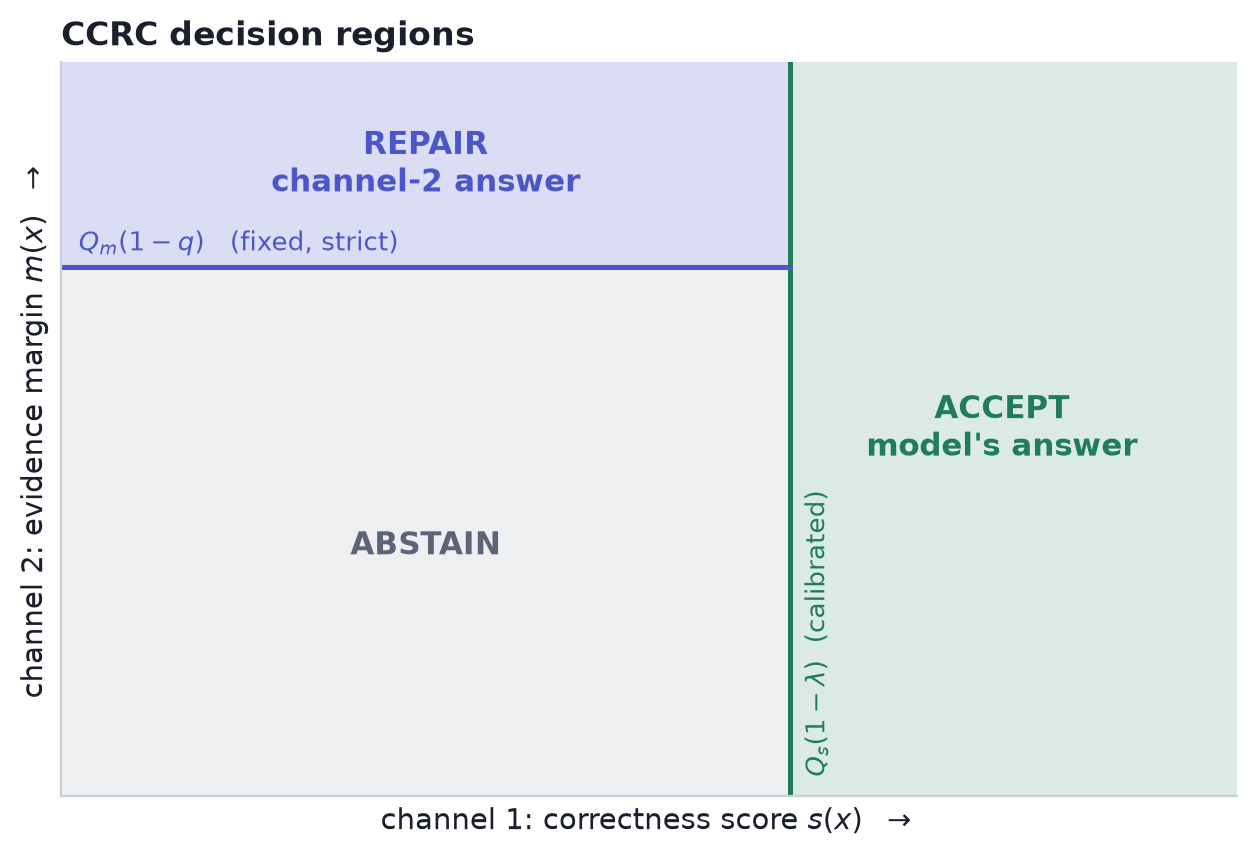
\includegraphics[width=0.62\textwidth]{fig_method.png}
\caption{CCRC partitions the $(s,m)$ plane. The acceptance threshold $Q_s(1-\lambda)$ is
calibrated; the repair gate $Q_m(1-q)$ is fixed in advance and strict, so that as $\lambda$
loosens the accepted region grows and the repair region shrinks. Keeping $q$ fixed is what
makes the family nested and lets a single fixed-sequence test suffice
(\S\ref{sec:decoupling}).}
\label{fig:method}
\end{figure}

\subsection{Worked examples on real data}
\label{sec:qualitative}

Before turning to aggregates, Figure~\ref{fig:qualitative} shows what the three decisions
look like on individual POPE images, with the actual channel-1 score, channel-2 detection
confidence, and resulting action for each. The three columns illustrate the regimes the
procedure is designed to separate.

In the \textsc{accept} column the model answers a straightforward existence question
confidently and correctly, the detector agrees, and the item is emitted unchanged; these
cases carry the bulk of the coverage. The \textsc{repair} column contains the cases that
motivate the method: LLaVA is asked whether a computer mouse is present, answers
``no'' with $p=0.21$, and is \emph{wrong} --- the mouse is there. Channel~1 correctly
assigns a low correctness score ($s=0.18$), which under a filtering policy would produce an
abstention and no answer at all. The detector, however, localises the object with confidence
$0.90$, comfortably inside the top evidence decile, so CCRC substitutes the detector's
answer and the item is emitted \emph{correctly}. This is the dilution effect of
\S\ref{sec:mechanism} in a single instance: a high-precision repair converts an item that
filtering would discard into a low-risk emitted item.

The \textsc{abstain} column shows the necessary complement. Here the model is wrong
\emph{and} the detector is also wrong, with weak evidence in both cases ($m=0.04$ and
$m=0.03$); the questions ask about a handbag and a truck that are not present, and neither
channel supplies a certifiable answer. Abstention is the correct action, and no amount of
substitution would help. The existence of a substantial population of such items is why
CCRC's gains are bounded by Proposition~\ref{prop:precondition} rather than being able to
recover the entire abstained mass.

\begin{figure}[t]
\centering
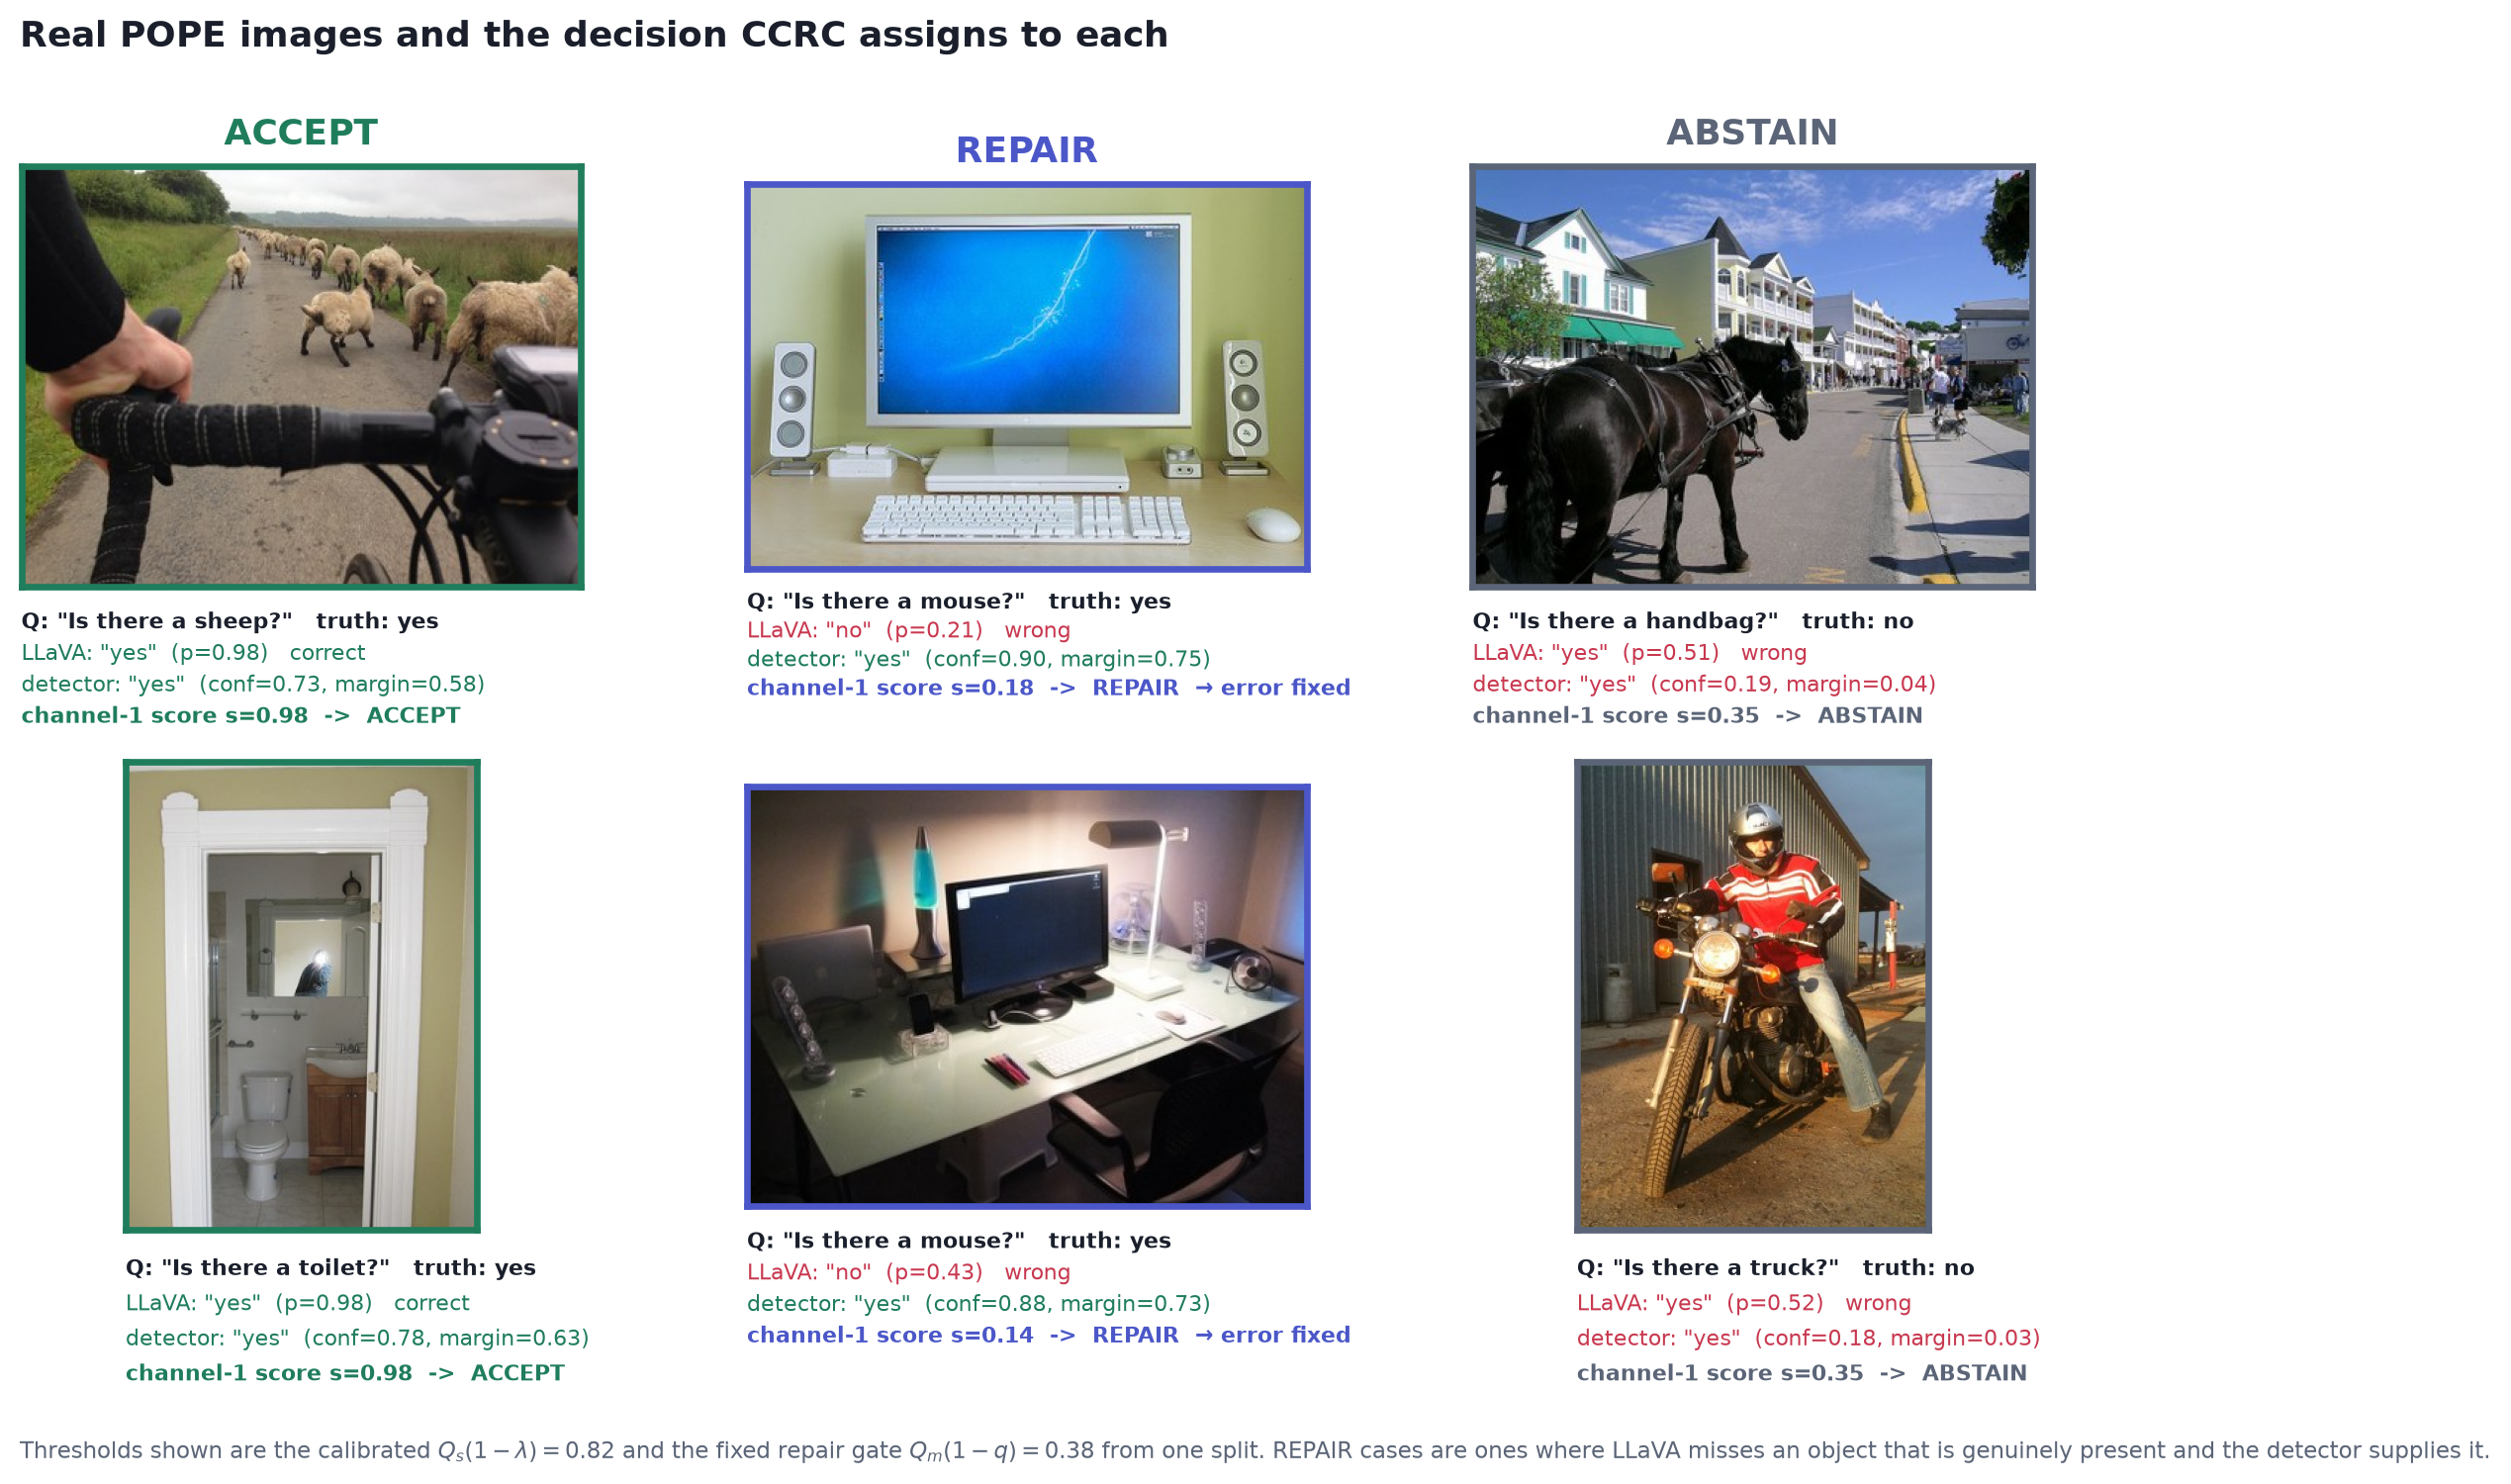
\includegraphics[width=\textwidth]{fig_qualitative.png}
\caption{Real POPE images with the actual quantities CCRC uses. Each panel reports the
question, the ground truth, LLaVA's answer with its probability, the detector's answer with
its confidence and evidence margin, the channel-1 correctness score, and the resulting
decision. \textbf{Accept} (left): both channels agree and the model is right.
\textbf{Repair} (centre): the model misses an object that is genuinely present and receives
a low correctness score, while the detector localises it with high confidence, so the
answer is substituted and the error is fixed --- items a filtering policy would abstain on.
\textbf{Abstain} (right): the model is wrong and the detector is also wrong with weak
evidence, so no certifiable answer exists and the procedure correctly declines. Thresholds
are the calibrated $Q_s(1-\lambda)$ and the fixed gate $Q_m(1-q)$ from one split.}
\label{fig:qualitative}
\end{figure}

\subsection{Validity}
\label{sec:validity}

\begin{theorem}[CCRC validity]
\label{thm:validity}
Let Assumptions~\ref{ass:exch}--\ref{ass:family} hold, let $\{\lambda_1<\dots<\lambda_M\}$
be a pre-specified grid, and let
\[
U(e,k;\delta)=\sup\{p:\Pr[\mathrm{Bin}(k,p)\le e]>\delta\}
\]
be the one-sided Clopper--Pearson upper confidence bound. Define
$\hat\lambda$ by fixed-sequence testing: proceed through $j=1,2,\dots$ while
$U(V_{\lambda_j},K_{\lambda_j};\delta)\le\alpha$ on the calibration fold, and set
$\hat\lambda$ to the last index that passed. Then the deployed policy
$\pi_{\hat\lambda}$ satisfies
\[
\Pr\bigl[\Risk(\emit_{\hat\lambda})\le\alpha\bigr]\ \ge\ 1-\delta .
\]
\end{theorem}

\begin{proof}
Fix $j$ and consider the null $H_j:\Risk(\emit_{\lambda_j})>\alpha$. Conditional on
$K_{\lambda_j}=k$, the emitted-set errors in \eqref{eq:err} are, under
Assumption~\ref{ass:exch}, exchangeable Bernoulli indicators; note that this holds for the
mixture because each emitted item contributes exactly one indicator, namely $1-Y_i$ if
accepted and $1-Y^{(2)}_i$ if repaired, and membership in $A_{\lambda_j}$ or $R_{\lambda_j}$
is determined by $(s,m)$ and the pre-specified $\lambda_j,q$ rather than by the labels.

Exchangeability alone does not give $V_{\lambda_j}\sim\mathrm{Bin}(k,\Risk)$, and the gap is
not academic in our implementation: $Q_s(1-\lambda)$ and $Q_m(1-q)$ are empirical quantiles
of the same fold whose errors are counted, so conditional on the calibration features the
emitted indicators have item-specific means and $V_{\lambda_j}$ is \emph{Poisson binomial}
with mean $k\bar p$, $\bar p=\Risk(\emit_{\lambda_j})$, rather than binomial.
Clopper--Pearson survives the substitution. The lower tail of a Poisson binomial with mean
$k\bar p$ is dominated by that of $\mathrm{Bin}(k,\bar p)$ \citep{hoeffding1956}, i.e.\
$\Pr[V_{\lambda_j}\le v]\le\Pr[\mathrm{Bin}(k,\bar p)\le v]$ for $v\le k\bar p$; and since
$U(v,k;\delta)$ is decreasing in $v$, the certification event
$\{U(V_{\lambda_j},k;\delta)\le\alpha\}$ is a lower-tail event on $V_{\lambda_j}$, so under
$H_j$ its probability is at most its probability under the equal-mean binomial. Hence, by
construction of the Clopper--Pearson bound, $\Pr[U(V_{\lambda_j},k;\delta)\le\alpha\mid H_j]\le\delta$: the event that the bound
certifies a policy whose true risk exceeds $\alpha$ has probability at most $\delta$, so
$p_j=\mathbf{1}\{U\le\alpha\}$ is a valid level-$\delta$ test of $H_j$.

The index set and its ordering are pre-specified by Assumption~\ref{ass:family}, which is
all that fixed-sequence testing requires for validity. Nesting is not needed for validity,
but it is what makes the procedure powerful: because $q$ is fixed, $A_\lambda$ increases and
$R_\lambda$ decreases in $\lambda$, so $\emit_\lambda=A_\lambda\cup M$ with
$M=\{m\ge Q_m(1-q)\}$ fixed, and \emph{coverage} is monotone increasing in $\lambda$ even
though the risk is not --- which is what makes ``the last index that passed'' the right thing
to return. Fixed-sequence testing applies: testing
$H_1,H_2,\dots$ in the pre-specified order and stopping at the first non-rejection controls
the family-wise error rate at $\delta$ without any multiplicity correction
\citep{angelopoulos2021ltt}. The returned $\hat\lambda$ is among the rejected hypotheses,
so with probability at least $1-\delta$ every rejected $H_j$ is false, i.e.
$\Risk(\emit_{\hat\lambda})\le\alpha$.
\end{proof}

\begin{remark}[why the mixture is not a complication]
The proof needs only that each emitted item contributes one $\{0,1\}$ error indicator whose
distribution does not depend on the labels of other items. Whether that indicator refers to
the model's answer or to channel~2's is irrelevant. This is precisely why
Proposition~\ref{prop:floor} does not bind: its premise restricts the \emph{action space},
which the guarantee itself does not require.
\end{remark}

\begin{lemma}[Minimum certifiable emitted-set size]
\label{lem:kmin}
With zero observed errors, $U(0,k;\delta)=1-\delta^{1/k}$. Hence no emitted set of size
$k$ can be certified at level $\alpha$ unless
\[
k\ \ge\ k_{\min}=\frac{\ln\delta}{\ln(1-\alpha)} .
\]
For $\alpha=\delta=0.10$, $k_{\min}=\lceil 21.85\rceil=22$.
\end{lemma}

\begin{proof}
$\Pr[\mathrm{Bin}(k,p)\le 0]=(1-p)^k$, so the upper bound with $e=0$ solves
$(1-p)^k=\delta$, giving $U(0,k;\delta)=1-\delta^{1/k}$. This is decreasing in $k$, and
$1-\delta^{1/k}\le\alpha\iff\delta^{1/k}\ge1-\alpha\iff k^{-1}\ln\delta\ge\ln(1-\alpha)$;
dividing by the negative quantity $\ln(1-\alpha)$ reverses the inequality and yields
$k\ge\ln\delta/\ln(1-\alpha)$. Since $U(e,k;\delta)\ge U(0,k;\delta)$ for $e\ge0$, no error
count can do better.
\end{proof}

Lemma~\ref{lem:kmin} is elementary but consequential: a fixed sequence whose first policy
emits fewer than $k_{\min}$ items fails at step one and, because fixed-sequence testing
stops at the first non-rejection, returns \emph{zero} coverage. We encountered exactly this
failure and now begin the grid at the analytically derived minimum.

\subsection{Why repairs cannot be self-certified in practice}
\label{sec:independence}

The most economical design would avoid a second channel: if $s$ says the model is probably
wrong, emit the opposite. This section shows why that fails. The argument has to be made at
the level of the \emph{mixture}, because that is what CCRC certifies --- a repair region
whose own risk exceeds $\alpha$ is not automatically inadmissible, since a compliant blend
can absorb it (Proposition~\ref{prop:dilution}). The correct statement is therefore not
that self-repair is impossible but that it is \emph{self-defeating}: the mass it can buy is
bounded by the accepted region's slack, and the fixed-sequence test aborts before it can be
collected.

\begin{proposition}[Self-repair is bounded by slack, and is not free]
\label{prop:selfrepair}
Suppose the answer space is binary and the repair is the negation of the model's answer, so
that $Y^{(2)}=1-Y$. Let $R\subseteq\mathcal{X}$ be any repair region with mass $c_r$ and let
the accepted region have mass $c_a$ and risk $r_a$. Then the risk of the repaired region is
\[
  r_r \;=\; \Pr[\text{repaired answer wrong}\mid X\in R] \;=\; \Pr[Y=1\mid X\in R],
\]
i.e.\ exactly the model's \textbf{accuracy} on $R$. Consequently, if $r_r>\alpha$ the
mixture is compliant only for
\begin{equation}
\label{eq:selfrepair}
  c_r \;\le\; c_a\,\frac{\alpha-r_a}{r_r-\alpha},
\end{equation}
and a region of accuracy $\le\alpha$ --- for which no such constraint binds --- requires the
score to isolate inputs on which the model is right less than $\alpha$ of the time. That is
strictly stronger than isolating inputs of low \emph{confidence}, and no monotone
transformation of $s$ can supply the difference.
\end{proposition}

\begin{proof}
On $R$ the emitted answer is $1-\hat a$, which is correct exactly when $\hat a$ is
incorrect; its error indicator is therefore $Y$, and averaging over $R$ gives
$r_r=\Pr[Y=1\mid X\in R]$. For the mixture,
$\bar r=(c_ar_a+c_rr_r)/(c_a+c_r)\le\alpha$ rearranges to
$c_r(r_r-\alpha)\le c_a(\alpha-r_a)$, which is \eqref{eq:selfrepair} when $r_r>\alpha$ and
is vacuous when $r_r\le\alpha$. The final claim follows because any repair rule of the form
$\{s(X)\le t\}$ has $r_r=\Pr[Y=1\mid s(X)\le t]$, a functional of the joint law of $(s,Y)$
invariant to monotone reparameterisation of $s$.
\end{proof}

Proposition~\ref{prop:selfrepair} converts an intuition --- ``a hallucination score reports
suspicion, not knowledge of the truth'' --- into a budget. Two measurements show how little
that budget buys.

\paragraph{No low-accuracy region exists where it is needed.}
Averaged over $60$ fits of the canonical score, the model's accuracy in the bottom $2\%$ of
$s$ is $20.9\%$ on POPE-1500 and $44.6\%$ on POPE-adversarial, against $\alpha=0.10$; in
the bottom decile it is $42.8\%$ and $47.3\%$. On Qwen2-VL the bottom $2\%$ is
\emph{above} chance at $64.3\%$, so flipping there is actively harmful. Only the two
settings with the lowest headroom (VCD-decoded LLaVA at $2.1\%$, AMBER at $0.0\%$) contain a
flippable region at all, and those are the settings with the least to gain.

\paragraph{The fixed sequence aborts before the slack can be spent.}
Substituting the negation of the model's answer at $q=0.02$ and certifying the mixture
exactly as in \S\ref{sec:validity}, certified coverage falls by $43.9$, $34.7$, $77.5$ and
$3.9$ points on the four POPE settings. The mechanism is not a graceful trade: the fixed
sequence returns \emph{nothing at all} on $65\%$, $88\%$, $100\%$ and $25\%$ of splits
respectively. The reason is structural. The self-repair region has fixed mass, so at the
\emph{start} of the grid --- where the accepted set is smallest and $K$ barely clears
$k_{\min}$ --- it is the largest fraction of the emitted set it will ever be, and its
$20$--$64\%$ error rate fails the very first hypothesis. Fixed-sequence testing must stop at
the first non-rejection (\S\ref{sec:validity}), so the procedure never reaches the later
$\lambda$ at which \eqref{eq:selfrepair} would in fact be satisfiable. Self-repair is
defeated by the interaction between a fixed-mass, high-error repair block and the prefix
structure of the test, not by the region being uncertifiable in isolation.

\paragraph{What this licenses us to claim.}
Not that certified correction is impossible without a second channel --- \eqref{eq:selfrepair}
admits self-repair whenever the accepted region has slack and the flip region is clean
enough, and on AMBER, where the bottom $2\%$ has $0\%$ accuracy, self-repair does gain
($+1.3$ points at $\alpha=0.10$). What the measurements license is the weaker and sufficient
claim that \emph{on the settings where filtering is expensive enough for correction to be
worth doing, no self-certifiable flip region exists}, so a second channel is required in
practice. We state this as an empirical regularity with a mechanism, not as a theorem, and
\S\ref{sec:discussion} lists it among the claims most likely to fail on a new benchmark.

Channel 2 escapes the budget in \eqref{eq:selfrepair} because $Y^{(2)}$ is a genuinely
different random variable, not a deterministic function of $Y$. Our detector is
$93$--$100\%$ accurate in its top evidence deciles (Table~\ref{tab:channel2}), so $r_r$
there is far below $\alpha$ and the constraint is vacuous rather than binding.

\begin{table}[t]
\centering
\caption{Channel-2 (detector) accuracy by evidence-margin decile on POPE. Repairs are drawn
only from the top decile, where accuracy is far above $1-\alpha$. Accuracy degrades broadly
with the margin, though not monotonically (the 8th decile falls slightly below the 6th),
which is why the repair gate must be strict rather than merely above the median.}
\label{tab:channel2}
\begin{tabular}{lccccc}
\toprule
Margin decile & 10th (top) & 9th & 8th & 6th & 1st (bottom)\\
\midrule
Detector accuracy & 1.000 & 0.960 & 0.927 & 0.934 & 0.513\\
\bottomrule
\end{tabular}
\end{table}

\subsection{Why the repair gate must be decoupled}
\label{sec:decoupling}

An earlier version of the procedure tied the repair gate to $\lambda$, i.e. used
$m(x)\ge Q_m(1-\lambda)$ in \eqref{eq:policy}. This is natural but harmful: as $\lambda$
loosens to admit more accepted items, the repair gate loosens in step and begins admitting
low-precision repairs, so the fixed sequence terminates earlier. Empirically the coupled
version gained on LLaVA ($+4.7$, $+5.3$ points) but \emph{lost} on Qwen2-VL ($-4.2$) and on
a VCD-decoded model ($-2.9$). It also required certifying two families (with and without
repair) at $\delta/2$ and selecting between them, wasting half the confidence budget.

Fixing $q$ removes both problems. The family becomes nested in the single parameter
$\lambda$, so one fixed-sequence test at full $\delta$ suffices
(Theorem~\ref{thm:validity}), and repair precision is held constant while $\lambda$ sweeps.
Table~\ref{tab:qsens} reports sensitivity: at $q=0.10$ the procedure gains in all eight
POPE-family cells, whereas looser gates can lose badly.

\begin{table}[t]
\centering
\caption{Sensitivity to the repair gate $q$: change in certified coverage relative to
filtering, over four settings $\times$ two risk levels. $q$ is fixed a priori, not tuned.}
\label{tab:qsens}
\begin{tabular}{lcc}
\toprule
Repair gate $q$ & Outcome across the eight cells & Worst cell\\
\midrule
$0.10$ (top decile)   & positive in all eight ($+0.5$ to $+8.0$) & $+0.5$\\
$0.25$                & mixed & $-16.3$\\
$0.50$                & mixed & $-15.5$\\
\bottomrule
\end{tabular}
\end{table}

\subsection{Why it gains: dilution and leverage}
\label{sec:mechanism}

Our initial hypothesis was that repairs \emph{spend} the accepted set's unused risk budget:
filtering typically realises a risk below $\alpha$ (we measure $8.0\%$ at $\alpha=0.10$),
and repairs with error above $\alpha$ could be admitted while the blend stayed compliant.
The measured effect runs the other way, and is stronger.

\begin{proposition}[Dilution lowers the emitted risk pointwise in $\lambda$]
\label{prop:dilution}
Fix $\lambda$ and let the accepted set have mass $c_a$ and risk $r_a$, and the repair set
mass $c_r$ and risk $r_r$. The emitted risk is the mixture
$\bar r=(c_ar_a+c_rr_r)/(c_a+c_r)$. If $r_r<r_a$ then $\bar r<r_a$, strictly decreasing in
$c_r$, so every $\lambda$ that is population-feasible for filtering remains
population-feasible with repairs and further $\lambda$ may become feasible. If instead
$r_r>\alpha>r_a$, admitting repairs consumes slack and may render feasible $\lambda$
infeasible.
\end{proposition}

\begin{proof}
$\bar r-r_a=c_r(r_r-r_a)/(c_a+c_r)$, which is negative iff $r_r<r_a$, and
$\partial\bar r/\partial c_r=c_a(r_r-r_a)/(c_a+c_r)^2$ has the same sign. Filtering is the
special case $c_r=0$, giving the feasibility claim. The last statement is the same
computation with the inequality reversed.
\end{proof}

\begin{remark}[Why this does not immediately imply a more permissive $\hat\lambda$]
\label{rem:prefix}
Proposition~\ref{prop:dilution} is a statement about the \emph{population} risk at fixed
$\lambda$, and two gaps separate it from the certified $\hat\lambda$ the procedure returns.
First, $\hat\lambda$ is chosen by a Clopper--Pearson bound on realised counts, not by
population feasibility: a single repaired item that happens to be wrong raises $V_\lambda$
and can tighten $\hat\lambda$ even when $r_r<r_a$. Second, fixed-sequence testing stops at
the first non-rejection, so a larger feasible \emph{set} yields a later stopping index only
if feasibility is a \emph{prefix} of the grid --- which is risk monotonicity in $\lambda$,
exactly what \S\ref{sec:validity} declines to assume. We therefore treat the coverage gain
as an empirical claim (\S\ref{sec:ccrcresults}) for which Proposition~\ref{prop:dilution}
supplies the mechanism, not a corollary. \S\ref{sec:independence} exhibits the failure mode
this remark anticipates: there, feasibility is not a prefix and the test aborts at the first
index.
\end{remark}

The empirically relevant regime is the first. Because repairs are drawn from the top
evidence decile, their risk is \emph{lower} than that of the acceptance gate's
\emph{marginal} items --- the items that determine whether the constraint binds. Repairs
therefore act as ballast: a small high-precision mass pulls $\bar r$ down and lets
$\lambda$ open further. The result is leverage.
Figure~\ref{fig:precondition}B plots it: $0.9$--$1.8\%$ of items repaired buys $1.9$--$4.7$
points of certified coverage --- per setting, ratios of $3.4\times$, $2.4\times$, $2.8\times$
and $1.9\times$.

\subsection{When it helps: a checkable precondition}
\label{sec:precondition}

CCRC is not a free improvement. Its upside is bounded by what filtering leaves on the
table, while its downside --- perturbing a nearly-saturated constraint --- is not
symmetrically bounded.

\begin{proposition}[Gain is capped by abstained mass]
\label{prop:precondition}
Let $\Cov_{\mathrm{filt}}$ be the coverage certified by filtering at level $(\alpha,\delta)$
and $\Cov_{\mathrm{CCRC}}$ that certified by CCRC. Then
\[
\Cov_{\mathrm{CCRC}}-\Cov_{\mathrm{filt}}\ \le\ 1-\Cov_{\mathrm{filt}},
\]
and $1-\Cov_{\mathrm{filt}}\ge(\mu-\alpha)/(1-\alpha)$ by
Proposition~\ref{prop:floor}. No matching lower bound on $\Cov_{\mathrm{CCRC}}$ holds, so
the upside is bounded by the abstained mass while the downside is not.
\end{proposition}

\begin{proof}
Coverage is at most one, so the gain cannot exceed the abstained fraction
$1-\Cov_{\mathrm{filt}}$; the floor inequality is Proposition~\ref{prop:floor} applied to
the filtering policy. The asymmetry claim follows because
Proposition~\ref{prop:dilution} shows the emitted risk strictly increases when repairs are
admitted with $r_r>r_a$, and Remark~\ref{rem:prefix} shows this can move $\hat\lambda$
downward without bound.
\end{proof}

\begin{remark}[Why this is a diagnostic and not a prediction]
\label{rem:notprediction}
An upper bound on the gain cannot predict a loss, and we previously overstated this. Write
$1-\Cov_{\mathrm{filt}}=(\mu-\alpha)/(1-\alpha)+\varepsilon$. One might hope $\varepsilon$
is small so that headroom $\mu-\alpha$ alone governs the achievable gain, but our own data
refutes it: on AMBER the floor is $1.6\%$ while $1-\Cov_{\mathrm{filt}}=7.9\%$, so
$\varepsilon=6.3\%$, four times the floor. The usable statement is therefore the crude one
--- the gain cannot exceed the abstained mass, so a setting that already certifies most of
its inputs has little to win and the same exposure to loss --- and the relationship between
headroom and realised gain is an empirical trend with visible exceptions
(\S\ref{sec:precondition}), not a law.
\end{remark}

Proposition~\ref{prop:precondition} predicts our one negative result. On AMBER's
discriminative split, $\mu=11.4\%$ against $\alpha=10\%$: the floor is $1.6\%$, filtering
already certifies $92.1\%$, and the theoretical headroom is at most $7.9$ points. Measured,
CCRC \emph{loses} $7.5$ points there. Figure~\ref{fig:precondition}A shows the gain tracking
$\mu-\alpha$ across all settings. Both quantities are known before calibration, so the
decision to deploy CCRC can be made a priori.

\begin{figure}[t]
\centering
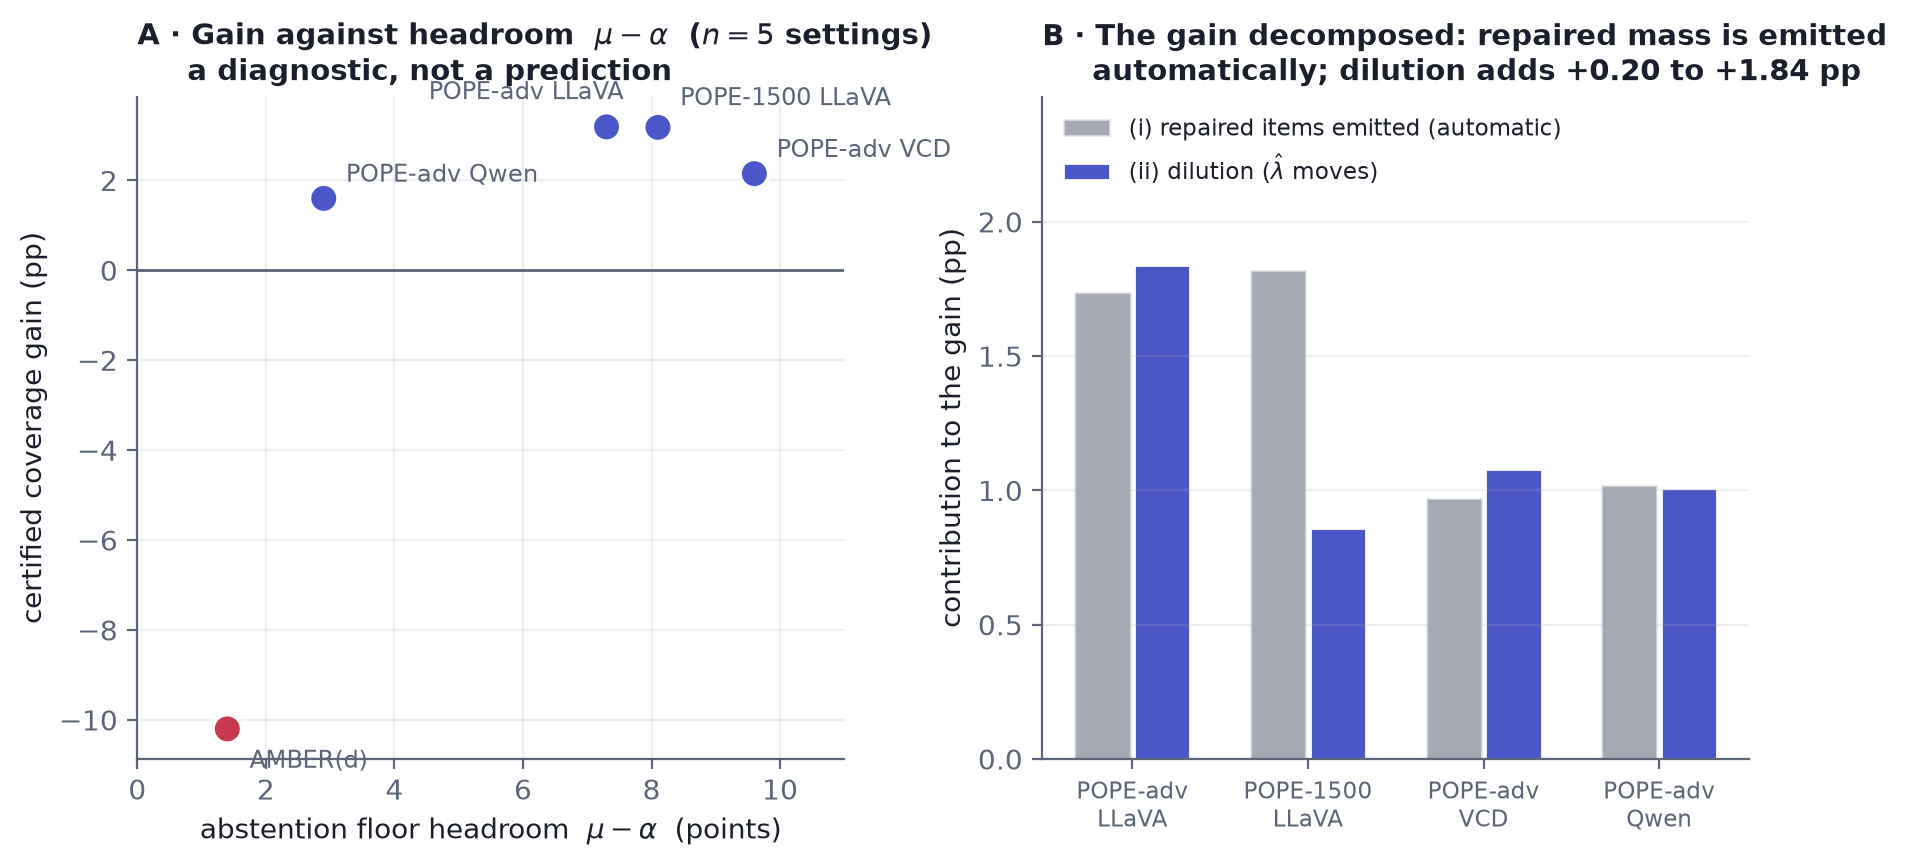
\includegraphics[width=\textwidth]{fig_precondition.png}
\caption{(A) Certified coverage gain against the abstention-floor headroom $\mu-\alpha$.
Gains appear when the headroom exceeds roughly three points and reverse when it does not:
AMBER(d), with $1.4$ points of headroom, is the single loss.
(B) Leverage: gain plotted against repaired mass, with $1\times$, $3\times$ and $6\times$
reference lines. A small high-precision repaired mass buys several times its own size in
coverage, consistent with the mechanism of Proposition~\ref{prop:dilution}.}
\label{fig:precondition}
\end{figure}

\subsection{Algorithm}

\begin{algorithm}[t]
\caption{CCRC (calibration and deployment)}
\label{alg:ccrc}
\begin{algorithmic}[1]
\Require folds $\mathcal{D}_{\mathrm{fit}},\mathcal{D}_{\mathrm{cal}}$ (disjoint), levels
$\alpha,\delta$, repair gate $q$, grid $\lambda_1<\dots<\lambda_M$ with
$\lambda_1$ chosen so $K_{\lambda_1}\ge k_{\min}$ (Lemma~\ref{lem:kmin}; our implementation
uses $\lambda_1=\min\{0.9,\max\{0.05,1.5k_{\min}/n_{\mathrm{cal}}\}\}$, the $1.5$ giving
headroom against fold-to-fold variation in $K$)
\State fit channel-1 score $s$ on $\mathcal{D}_{\mathrm{fit}}$ \Comment{disjoint from
calibration; see \S\ref{sec:ablations}}
\State $t_m\gets Q_m(1-q)$ on $\mathcal{D}_{\mathrm{cal}}$ \Comment{repair gate fixed}
\State $\hat\lambda\gets\varnothing$
\For{$j=1$ to $M$}
  \State $A\gets\{i\in\mathcal{D}_{\mathrm{cal}}:s_i\ge Q_s(1-\lambda_j)\}$;
         $R\gets\{i\notin A:m_i\ge t_m\}$
  \State $V\gets\sum_{i\in A}(1-Y_i)+\sum_{i\in R}(1-Y^{(2)}_i)$; $K\gets|A|+|R|$
  \If{$K<k_{\min}$} \textbf{continue} \Comment{uncertifiable by Lemma~\ref{lem:kmin}; not
         evidence against $H_j$}
  \ElsIf{$U(V,K;\delta)\le\alpha$} $\hat\lambda\gets\lambda_j$
  \Else\ \textbf{break} \Comment{fixed-sequence testing stops at the first non-rejection}
  \EndIf
\EndFor
\State \textbf{at test time, for input $x$:} \textbf{if} $\hat\lambda=\varnothing$ abstain on
  every input (coverage $0$);
  \textbf{else if} $s(x)\ge Q_s(1-\hat\lambda)$ emit $\hat a(x)$;
  \textbf{else if} $m(x)\ge t_m$ emit $b(x)$;
  \textbf{else} abstain
  \Statex \Comment{$Q_s,Q_m$ are the calibration-fold quantiles fixed above, not recomputed
  at test time}
\end{algorithmic}
\end{algorithm}

%===============================================================================
\section{Experiments}
\label{sec:exp}

\paragraph{Protocol.}
Every reported number uses a three-way disjoint split --- fit the score, calibrate the
threshold, test --- with fixed-sequence testing and Clopper--Pearson bounds at
$\delta=0.10$, averaged over $20$--$100$ random splits. The three-way split is not cosmetic:
\S\ref{sec:ablations} shows that reusing the calibration fold to fit the score silently
breaks the guarantee for high-capacity scores.

\paragraph{How validity is audited.}
Mean realised risk is \emph{not} the guarantee. The claim is
$\Pr[\Risk\le\alpha]\ge1-\delta$, so the quantity to audit is the fraction of calibration
draws whose risk exceeds $\alpha$, compared against $\delta$. We report both, and we
distinguish two versions of the former, because realised risk on a finite test fold carries
binomial noise that is not a validity failure. Scored on the test fold, exceedance is
$11$--$15\%$ on the POPE settings against $\delta=0.10$; scored on the full item set --- a
lower-noise proxy for the population risk of the selected policy --- it is $1$--$4\%$. The
guarantee holds; the discrepancy is finite-sample noise in the audit, and we flag it because
the naive statistic looks like a violation and the mean-risk statistic hides both.

\paragraph{Models and data.}
Backbones are LLaVA-1.5-7B \citep{llava} in 4-bit and Qwen2-VL-2B-Instruct \citep{qwenvl};
we additionally evaluate LLaVA decoded with visual contrastive decoding \citep{vcd}.
Channel 2 is OWLv2-base \citep{owlv2}. Benchmarks are POPE \citep{pope} (random and
adversarial splits), AMBER discriminative \citep{amber}, MME \citep{mme}, GQA \citep{gqa}
and HallusionBench \citep{hallusionbench}. All per-item extracted signals are released so
that the analyses can be reproduced without a GPU.

\subsection{The correctness score}
\label{sec:score}

Validity holds for any score; only efficiency depends on which one is used. We therefore
first characterise what makes a score efficient here.

Table~\ref{tab:score} compares scores on POPE. A learned combination of the model's own
confidence signals is a solid baseline. Generic image--text similarity \citep{clip} adds
little. An open-vocabulary \emph{detection} signal adds a great deal: $+8.4$ points of
certified coverage against $+2.3$ for CLIP.

\begin{table}[t]
\centering
\caption{Selective prediction on POPE (LLaVA-1.5-7B, $n=1500$). AURC is area under the
risk--coverage curve (lower better). Realised test risk was $\le\alpha$ in every row.}
\label{tab:score}
\begin{tabular}{lccc}
\toprule
Score & AURC $\downarrow$ & cov@$10\%$ $\uparrow$ & AUROC $\uparrow$\\
\midrule
Raw confidence                      & 0.0798 & 62.0\% & 0.762\\
Learned, confidence only            & 0.0701 & 63.6\% & 0.782\\
\quad + CLIP grounding \citep{clip} & 0.0650 & 66.0\% & 0.796\\
\quad + detection grounding \citep{owlv2} & \textbf{0.0566} & \textbf{73.1\%} & \textbf{0.829}\\
\quad + both                        & 0.0559 & 74.1\% & 0.831\\
\bottomrule
\end{tabular}
\end{table}

Against a baseline given \emph{both} confidence and multi-sample self-consistency --- the
scoring philosophy of \citet{conflvlm} --- detection grounding still adds
$11.9\pm21.1$ points on the adversarial split (Table~\ref{tab:selfcons}) --- a mean gain in
the same direction, but with a standard deviation that swamps it. We flag this rather than
report it as support: with $n=450$ a three-way split leaves a $150$-item calibration fold,
which is genuinely underpowered for a Clopper--Pearson bound at $\delta=0.10$, and the wide
interval reflects that rather than an absence of grounding signal. The POPE-1500 result
($+9.6\pm4.7$) is the one we would rely on.

\begin{table}[t]
\centering
\caption{Against a faithful self-consistency baseline on POPE-adversarial, the hardest
split ($K=3$ samples, LLaVA-1.5, $n=450$).}
\label{tab:selfcons}
\begin{tabular}{lcc}
\toprule
Score & AURC $\downarrow$ & cov@$10\%$ $\uparrow$\\
\midrule
Self-consistency only & 0.147 & 0.0\%\\
Confidence $+$ self-consistency & 0.082 & 45.8\%\\
\quad $+$ detection grounding (ours) & \textbf{0.063} & \textbf{57.7\%}\\
\bottomrule
\end{tabular}
\end{table}

Two regularities follow. The advantage of grounding \emph{grows as the guarantee tightens}:
at $\alpha=0.05$ it nearly doubles usable coverage ($26.4\%\to47.1\%$), while at
$\alpha=0.20$ both scores certify almost everything (Figure~\ref{fig:covalpha}). And the
advantage tracks how much the base model hallucinates: on the more accurate Qwen2-VL-2B the
same addition is worth $2.0$ points rather than $11.9$, both with intervals that include zero. Grounding is most valuable exactly
where selective prediction is most expensive.

\begin{figure}[t]
\centering
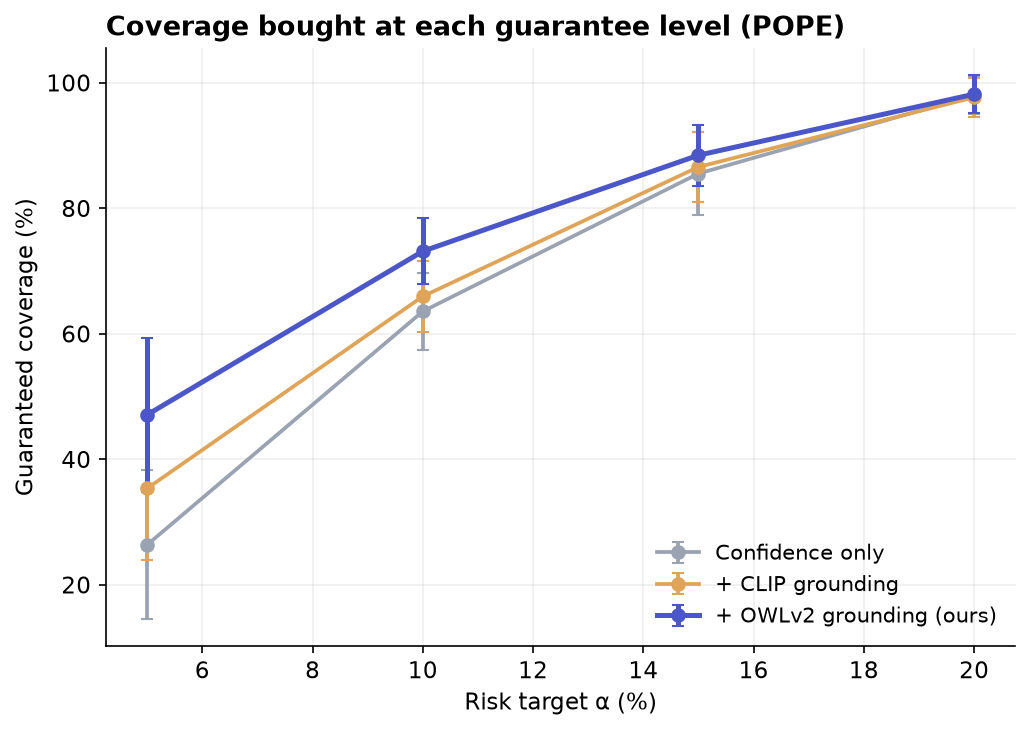
\includegraphics[width=0.62\textwidth]{coverage_vs_alpha.png}
\caption{Certified coverage as a function of the risk target. The grounded score dominates
at every level and the margin widens as $\alpha$ tightens; at $\alpha=0.05$ it nearly
doubles coverage. Error bars are one standard deviation over splits.}
\label{fig:covalpha}
\end{figure}

\begin{remark}[accuracy is not separability]
\label{rem:sep}
A detector whose standalone accuracy matches the VLM's on POPE ($83.1\%$ vs.\ $81.9\%$)
certifies far less coverage when used as a selective predictor in its own right
($55.3\%$ vs.\ $68.2\%$). Conformal coverage depends on how well a score \emph{separates}
correct from incorrect outputs, not on how often the underlying predictor is right. This
also answers the natural objection to CCRC --- ``if channel 2 is good, why not just use
it?'' --- in three of four settings (Table~\ref{tab:baselines}).
\end{remark}

\subsection{CCRC across settings}
\label{sec:ccrcresults}

Table~\ref{tab:ccrc} reports CCRC against filtering under an identical protocol. The
guarantee holds in every row. Gains are $+0.5$ to $+8.0$ points where the diagnostic of
\S\ref{sec:precondition} is satisfied, and the single violation of that precondition is
also the single loss.

\begin{table}[t]
\centering
\caption{CCRC ($q{=}0.10$) versus filtering. Realised test risk was $\le\alpha$ in every
row; realised risk for every row is reported in Table~\ref{tab:multialpha} and. The final row violates the precondition of
Proposition~\ref{prop:precondition} and is the only loss.}
\label{tab:ccrc}
\begin{tabular}{llcccccc}
\toprule
Dataset & Backbone & $n$ & $\mu$ & $\alpha$ & Filter & CCRC & Gain\\
\midrule
POPE            & LLaVA-1.5    & 1500 & 18.1\% & 0.10 & 68.2\% & \textbf{72.6\%} & $+4.4$\\
POPE-adv        & LLaVA-1.5    & 444  & 17.3\% & 0.10 & 42.1\% & \textbf{46.8\%} & $+4.7$\\
POPE-adv        & Qwen2-VL-2B  & 591  & 12.9\% & 0.10 & 77.5\% & \textbf{79.4\%} & $+1.9$\\
POPE-adv        & LLaVA+VCD    & 591  & 19.6\% & 0.10 & 45.0\% & \textbf{47.5\%} & $+2.5$\\
\midrule
POPE            & LLaVA-1.5    & 1500 & 18.1\% & 0.15 & 86.8\% & \textbf{88.4\%} & $+1.7$\\
POPE-adv        & LLaVA-1.5    & 444  & 17.3\% & 0.15 & 69.2\% & \textbf{77.2\%} & $+8.0$\\
POPE-adv        & Qwen2-VL-2B  & 591  & 12.9\% & 0.15 & 94.4\% & \textbf{94.9\%} & $+0.5$\\
POPE-adv        & LLaVA+VCD    & 591  & 19.6\% & 0.15 & 73.4\% & \textbf{75.4\%} & $+2.0$\\
\midrule
AMBER(d)        & LLaVA-1.5    & 228  & 11.4\% & 0.10 & 92.1\% & 84.5\% & $-7.5$\\
\bottomrule
\end{tabular}
\end{table}

\paragraph{Isolating the cause of the AMBER loss.}
Two candidate explanations were tested and rejected. It is not a weak repair channel: the
detector is $95.6\%$ accurate on that dataset overall and $100\%$ accurate in the top-decile
region repairs are drawn from. It is not small sample size: subsampling POPE to the same
$n=228$ still gains $+3.2$ points, and the gain grows with $n$ ($+5.6$ at $400$, $+10.3$ at
$700$). The cause is the absence of headroom, exactly as Proposition~\ref{prop:precondition}
predicts.

\subsection{Where grounding does not apply}
\label{sec:exp:noapply}

Benchmark composition determines whether channel 2 exists at all.
Table~\ref{tab:datasets} reports the full sweep. On MME's full split, GQA's yes/no subset
and HallusionBench, the questions are largely about attributes, counting or reasoning, so no
object can be extracted for the detector to check; the procedure reduces to filtering, which
remains valid. HallusionBench is instructive: LLaVA scores $51.2\%$, essentially chance, and
the certified coverage is $0.0\%$. That is the guarantee working as intended --- with
$\mu\approx0.49$ and $\alpha=0.10$, Proposition~\ref{prop:floor} forces abstention on at
least $43\%$ of inputs, and in practice on all of them.

\begin{table}[t]
\centering
\begin{threeparttable}
\caption{Full dataset sweep. ``grnd'' indicates whether channel 2 applies. Coverage columns
are confidence-only $\to$ with grounding, at $\alpha=0.10$.}
\label{tab:datasets}
\begin{tabular}{llccc}
\toprule
Dataset & Backbone & acc & grnd & cov@$10\%$\\
\midrule
POPE ($1500$)     & LLaVA-1.5   & 81.9\% & yes & $63.6\to\mathbf{73.1}$\%\\
POPE-adv          & LLaVA-1.5   & 82.7\% & yes & $46.6\to\mathbf{57.4}$\%\\
POPE-adv          & Qwen2-VL-2B & 87.3\% & yes & $83.5\to\mathbf{85.5}$\%\\
POPE-adv          & LLaVA+VCD   & 80.3\% & yes & $21.8\to\mathbf{53.9}$\%\\
MME-existence\tnote{a} & LLaVA-1.5 & 95.0\% & yes & underpowered\\
AMBER(d)          & LLaVA-1.5   & 78.6\% & partial & see Table~\ref{tab:ccrc}\\
MME (full)        & LLaVA-1.5   & 68.9\% & no  & $5.7$\%\\
GQA (yes/no)      & LLaVA-1.5   & 72.4\% & no  & $17.8$\%\\
HallusionBench    & LLaVA-1.5   & 51.2\% & no  & $0.0$\%\\
\bottomrule
\end{tabular}
\begin{tablenotes}
\item[a] Only $60$ items, leaving a $20$-item calibration fold under the three-way split,
which is below $k_{\min}=22$ (Lemma~\ref{lem:kmin}). Sample size is not the only
obstruction: at this subset's low base error rate $U(3,60;\delta)=0.108>\alpha$, so power
would bind even with the full $60$ items available for calibration.
\end{tablenotes}
\end{threeparttable}
\end{table}

\subsection{Composition with a mitigation decoder}
\label{sec:vcd}

Because the two programmes of \S\ref{sec:related} are orthogonal --- mitigation lowers
$\mu$, risk control governs what is emitted --- our layer should compose with a mitigation
decoder. It does, and most strongly where the decoder's own confidence is poorly
calibrated. On POPE-adversarial with visual contrastive decoding \citep{vcd}, adding
grounding improves AURC from $0.1030$ to $0.0603$ and certified coverage from $47.6\%$ to
$64.2\%$ ($\Delta\text{AURC}=0.043\pm0.007$).

\subsection{Baselines and attribution}
\label{sec:attribution}

\paragraph{Detector alone.}
Table~\ref{tab:baselines} answers Remark~\ref{rem:sep}'s objection directly. CCRC beats a
detector-only selective predictor in three of four settings, sometimes by very large
margins, because the detector's correctness is harder to \emph{score} than the VLM's. Where
the detector genuinely dominates the VLM in accuracy (AMBER: $95.6\%$ vs.\ $88.6\%$) it also
wins standalone, which is a second reason CCRC is the wrong tool in that regime.

\begin{table}[t]
\centering
\caption{Detector-only selective prediction versus CCRC ($\alpha=0.10$, identical protocol).}
\label{tab:baselines}
\begin{tabular}{lccccc}
\toprule
Setting & VLM acc & det.\ acc & Filter (VLM) & CCRC & Detector only\\
\midrule
POPE-1500 LLaVA   & 81.9\% & 83.1\% & 68.2\% & \textbf{72.6\%} & 55.3\%\\
POPE-adv LLaVA    & 82.7\% & 82.4\% & 42.1\% & \textbf{46.8\%} & 13.0\%\\
POPE-adv Qwen2-VL & 87.1\% & 82.9\% & 77.5\% & \textbf{79.4\%} & 21.8\%\\
AMBER(d) LLaVA    & 88.6\% & 95.6\% & 92.1\% & 84.5\% & \textbf{92.6\%}\\
\bottomrule
\end{tabular}
\end{table}

\paragraph{A published scorer, and where our margin comes from.}
Table~\ref{tab:attrib} places the CLIP-similarity scoring function of \citet{conflvlm} in
our pipeline and adds our components one at a time. The aggregate margin is $+67$ points,
and reporting only that number would misattribute it: $+62.6$ of the $67$ comes from the
score, and $+4.4$ from certified correction. We also note the comparison understates
\citet{conflvlm}, whose method was designed for free-form caption claims rather than yes/no
probes; we transplant their scorer, not their system.
Figure~\ref{fig:riskcov} shows the corresponding risk--coverage curves.

\begin{table}[t]
\centering
\caption{Attribution on POPE ($\alpha=0.10$). Most of the margin over a published scorer
comes from the score, not from our procedure.}
\label{tab:attrib}
\begin{tabular}{lcc}
\toprule
Method & Coverage & $\Delta$\\
\midrule
CLIP-similarity scorer \citep{conflvlm}, filtering & 5.6\%  & ---\\
\quad + VLM confidence                             & 41.5\% & $+35.9$\\
\quad + detection grounding                        & 68.2\% & $+26.7$\\
\quad + certified correction (CCRC)                & \textbf{72.6\%} & $+4.4$\\
\bottomrule
\end{tabular}
\end{table}

\begin{figure}[t]
\centering
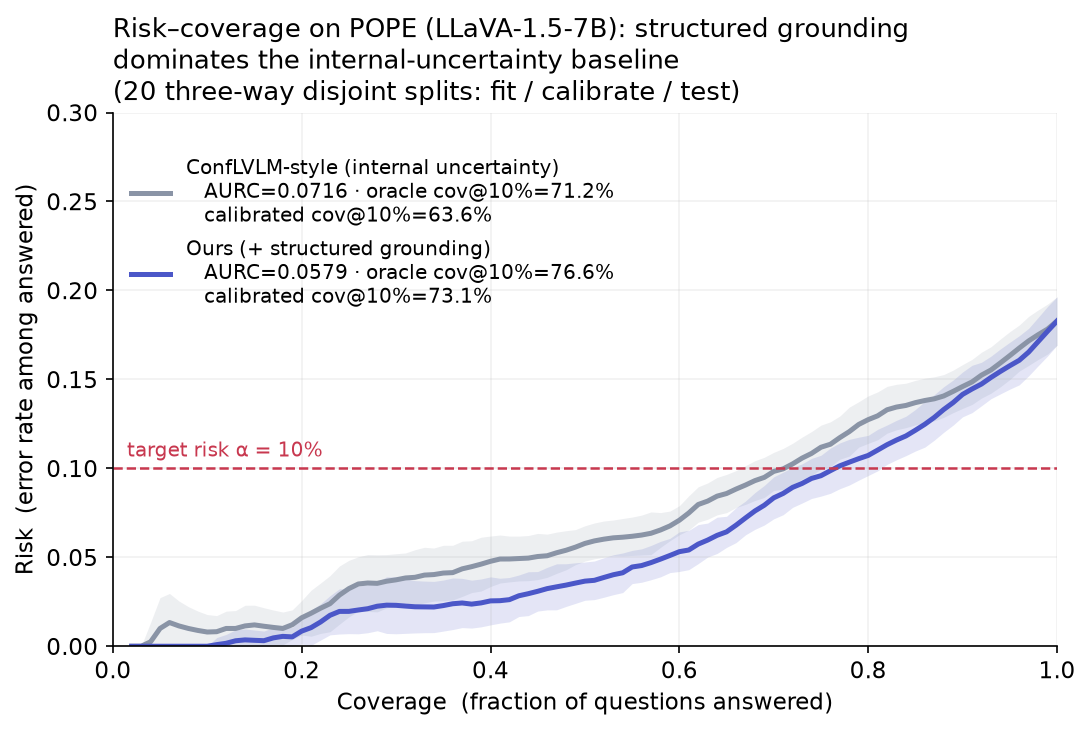
\includegraphics[width=0.72\textwidth]{risk_coverage.png}
\caption{Risk--coverage curves on POPE. The grounded score (blue) lies below the
confidence-only baseline (LLaVA's own logits, no external evidence) at every coverage level
short of full coverage, where both necessarily meet the base risk: lower error for the same
coverage, and more coverage for the same error target. Shaded bands are one standard
deviation over $20$ three-way splits; the dashed line marks $\alpha=0.10$. The legend
reports two quantities that should not be confused: \emph{oracle} coverage read off the
test-fold curve ($71.2\%\to76.6\%$), and conformally \emph{calibrated} coverage
($63.6\%\to73.1\%$), the latter being what the tables report. Note that this baseline is not
ConfLVLM: ConfLVLM's scorer is CLIP image--text similarity, which appears here as the
``$+$ CLIP grounding'' arm of Figure~\ref{fig:comparison} and as a separate row of
Table~\ref{tab:score}.}
\label{fig:riskcov}
\end{figure}

\paragraph{The closest concurrent method.}
\label{sec:bcea}
\citet{bcea} rescue borderline claims by acquiring zoomed views and re-scoring the
\emph{original} assertion. Holding the base score fixed and adding one mechanism per arm
(Table~\ref{tab:bcea}), the two mechanisms are complementary: composing them beats every
single-mechanism arm at both risk levels. Re-reading the image and replacing the answer
rescue different claims. We do not claim to beat \citet{bcea}: our reproduction uses three
coarse crops and under-delivers relative to their published gain at $\alpha=0.10$, so the
defensible conclusion is composition, not superiority.

\begin{table}[t]
\centering
\caption{One common base score, one mechanism added per arm (POPE, LLaVA-1.5, $n=394$
grounded items). All arms valid. Composition beats every single mechanism.}
\label{tab:bcea}
\begin{tabular}{lcc}
\toprule
Arm & cov@$0.10$ & cov@$0.15$\\
\midrule
Base filter (confidence only)              & 5.5\%  & 16.5\%\\
\quad + evidence acquisition \citep{bcea}  & 5.5\%  & 24.1\%\\
\quad + detection-grounded score (ours)    & 32.1\% & 63.2\%\\
\quad + certified correction (ours)        & 34.5\% & 71.8\%\\
\textbf{Composed}                          & \textbf{35.8\%} & \textbf{74.2\%}\\
\bottomrule
\end{tabular}
\end{table}

%===============================================================================
\section{A sequential failure mode}
\label{sec:sequential}

Correction is more attractive in free-form generation than in yes/no answering: replacing a
hallucinated word preserves a caption that deletion would mutilate. The extension looks
mechanical --- decompose the caption into claims, repair the unsupported ones, continue
decoding --- and two obstacles are already known. Editing a prefix makes later tokens
off-policy, which is feedback covariate shift rather than exogenous shift
\citep{fannjiang2022fcs}, so weighted conformal methods \citep{tibshirani2019} do not apply.
And per-claim guarantees say nothing about a whole sequence, whose length is itself
data-dependent.

Both could in principle be handled. Prefix-conditional (Mondrian) $p$-values make each
decision valid given the realised prefix, so how we arrived there --- including by our own
edits --- is absorbed into the conditioning; e-processes with Ville's inequality give
sequence-level anytime validity, and are robust to adaptive intervention because our
corrections are predictable with respect to the decoding filtration
\citep{waudbysmith2024,ramdas2023}. The residual difficulty is that the calibration pool
drifts, since the deployed policy writes different text. The natural fix is on-policy
calibration by iteration to a fixed point, and its convergence argument requires the
correction map to be monotone. We measured whether it is, before attempting a proof.

\paragraph{Design.}
For each image we generate a caption greedily, locate the first hallucinated object mention
at position $t$ using AMBER's per-image present/absent object lists, and construct two
prefixes \emph{identical up to $t$}: one retaining the hallucinated word, one substituting
the best-detected object the image genuinely contains. We then continue decoding the same
number of tokens from each prefix and count hallucinated mentions in the continuations
only. Matched prefixes make the contrast causal: the only difference between the two
continuations is the intervention.

\paragraph{Result.}
Repair makes the continuation worse (Table~\ref{tab:monotone},
Figure~\ref{fig:monotonicity}). Downstream hallucinated mentions rise from $1.207$ to
$1.413$, a paired difference of $+0.207\pm0.091$ ($n=121$, $t=2.27$, $p=0.025$; Wilcoxon
$p=0.035$), with $45$ cases worsening against $25$ improving.

\begin{table}[t]
\centering
\caption{Paired matched-prefix test of monotonicity ($n=121$ cases). Repair significantly
increases hallucination in the continuation.}
\label{tab:monotone}
\begin{tabular}{lcc}
\toprule
Downstream measure (continuation only) & Original prefix & Repaired prefix\\
\midrule
Hallucinated mentions (mean)      & 1.207 & \textbf{1.413}\\
Hallucinations per 100 words      & 3.61  & 4.30\\
Faithful mentions (mean)          & 1.579 & 1.752\\
Continuation length (words)       & 33.4  & 32.9\\
\midrule
\multicolumn{3}{l}{Paired difference $+0.207\pm0.091$; $t=2.27$, $p=0.025$; Wilcoxon $p=0.035$}\\
\multicolumn{3}{l}{Cases better / worse / tie: $25$ / $45$ / $51$}\\
\bottomrule
\end{tabular}
\end{table}

\begin{figure}[t]
\centering
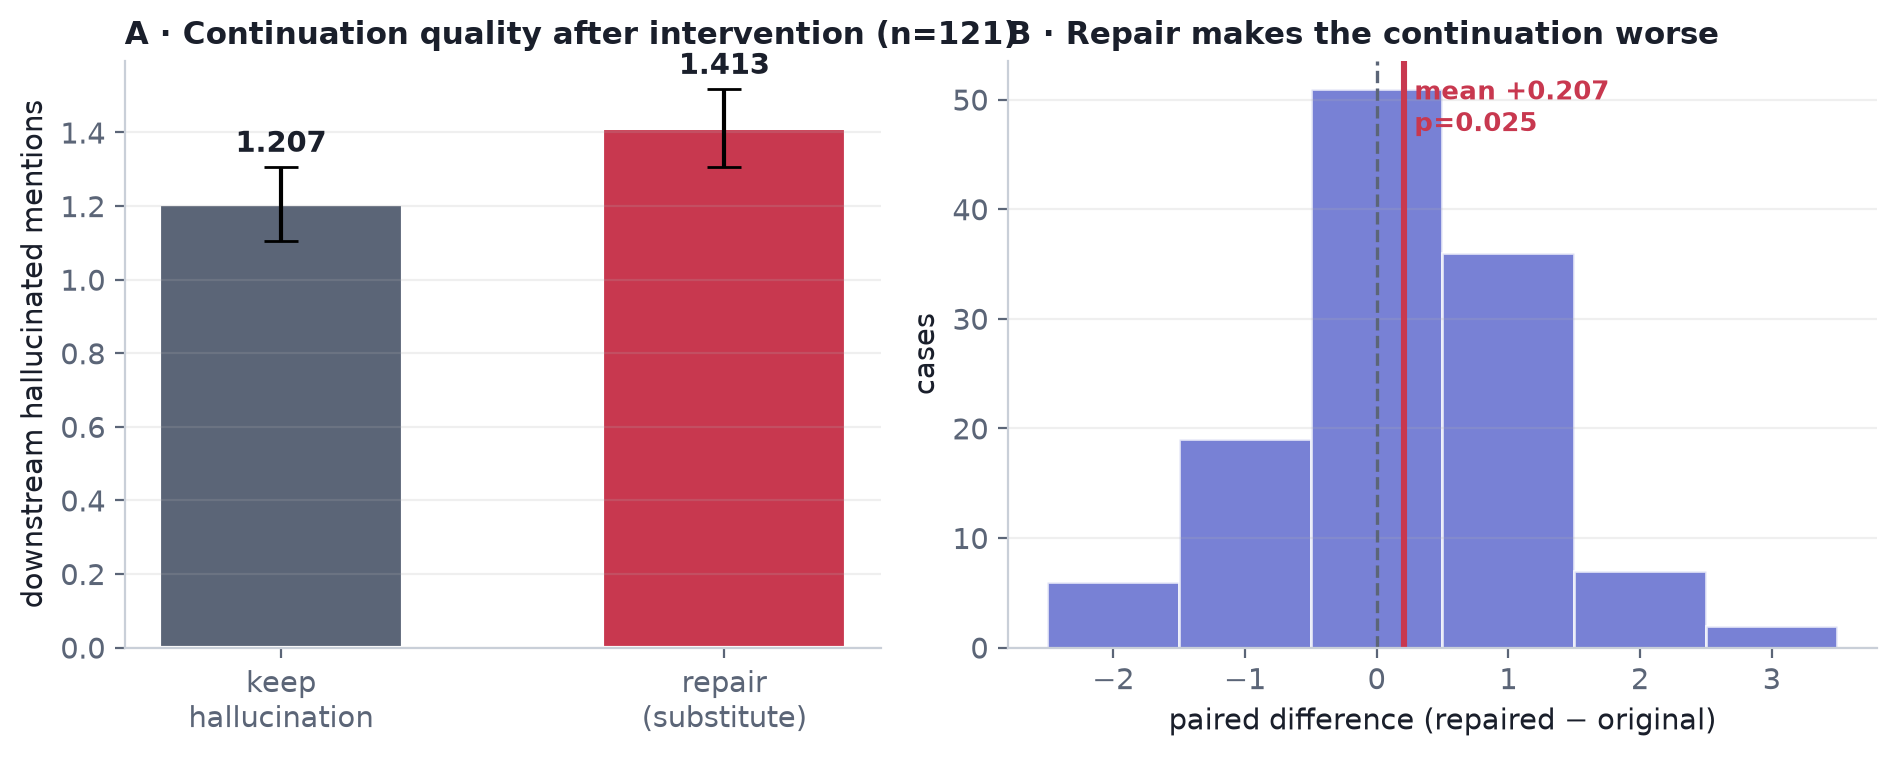
\includegraphics[width=\textwidth]{fig_monotonicity.png}
\caption{(A) Mean hallucinated mentions in the continuation after keeping versus repairing
the flagged claim; error bars are standard errors. (B) Distribution of the paired
difference; mass to the right of zero indicates repair worsening the continuation. The
effect is modest in size but statistically clear, and its sign is what matters for the
theory.}
\label{fig:monotonicity}
\end{figure}

\paragraph{What this rules out.}
The correction map is not monotone, so the fixed-point argument has no basis: monotone
convergence arguments of Knaster--Tarski type do not apply, and iterating calibration and
deployment need not converge. We therefore do not claim a sequential guarantee of that
form. What survives is a coupling bound, which is weaker but assumption-light.

For a sequence of claims $O=(o_1,\dots,o_T)$ let $\Risk(O)=\E[\,\#\{t:o_t\text{ false}\}\,]$
be the expected count of false claims, the quantity a CHAIR-style loss charges for. Two
regimes must be separated, and the distinction is exactly what \S\ref{sec:sequential}
measures.

\begin{theorem}[Coupling bound for corrected outputs]
\label{thm:coupling}
Let $O$ denote the original output and $O'$ the output after a repair rule is applied to a
region $R$, and suppose the repair is \emph{non-interfering}: conditional on not being
repaired, every claim's truth value is unchanged by repairs elsewhere. Then
\[
\Risk(O')\ \le\ \Risk(O)\;+\;\Pr[X\in R]\cdot\Pr[\text{repair wrong}\mid X\in R].
\]
Without non-interference the bound acquires a third term,
\begin{equation}
\label{eq:interference}
\Risk(O')\ \le\ \Risk(O)\;+\;\Pr[X\in R]\cdot\Pr[\text{repair wrong}\mid X\in R]\;+\;\Iota,
\qquad \Iota \;:=\; \E\big[\Delta_{R^c}\big],
\end{equation}
where $\Delta_{R^c}$ is the change in the number of false claims outside $R$ induced by
repairing inside it.
\end{theorem}

\begin{proof}
Decompose by whether a claim is repaired. Under non-interference the claims in $R^c$ retain
their truth values, contributing at most $\Risk(O)$; on $R$ the emitted claim is wrong only
if the repair is wrong, contributing at most
$\Pr[X\in R]\Pr[\text{repair wrong}\mid X\in R]$. Summing gives the first bound. In general
the $R^c$ contribution is $\Risk(O)+\E[\Delta_{R^c}]$ by definition of $\Delta_{R^c}$, which
gives \eqref{eq:interference}.
\end{proof}

\begin{remark}[The interference term is not negligible here]
\label{rem:interference}
Non-interference is the assumption \S\ref{sec:sequential} falsifies: we measure
$\widehat{\Iota}=+0.207\pm0.091$ additional false claims per repair ($n=121$, $p=0.025$), so
for a single repair the interference term is roughly the same size as the direct repair-error
term and cannot be dropped. Any procedure certifying corrected sequences must estimate
$\Iota$ rather than assume it away, and $\Iota$ depends on the repair rule --- which is why
a context-aware rule is the natural next step rather than a tighter bound.
\end{remark}

\begin{remark}[What the corollary does and does not give]
\label{rem:corollary}
Controlling $\Risk(O)\le\alpha_1$ and the repair term by $\alpha_2$ at confidence
$1-\delta/2$ each yields $\Risk(O')\le\alpha_1+\alpha_2+\Iota$ at confidence $1-\delta$. We
flag a limitation of this composition rather than hiding it: certifying $\Risk(O)$ for the
\emph{uncorrected} generation is precisely the object the abstention floor makes expensive,
so the corollary is useful only relative to an already-selective base policy (for which
$\Risk$ is conditioned on emission), not to raw generation. Making the sequential guarantee
self-contained --- certifying the corrected sequence without first certifying the
uncorrected one --- remains open.
\end{remark}

\paragraph{What this implies for algorithm design.}
Beyond closing off a proof strategy, the measurement identifies a cost that a myopic
procedure does not charge for. Greedy per-claim repair optimises the risk of the claim in
front of it while imposing roughly $0.21$ additional hallucinated claims on the
continuation. A correct sequential procedure must therefore price the \emph{continuation},
not the claim --- for instance by searching over rewrite trajectories under an accumulated
risk ledger rather than deciding each claim independently. We regard this as the main open
problem the paper leaves, and note that it is a genuinely different statistical object:
because repairing claim $i$ changes which claims $i+1,\dots$ exist, the item set is
endogenous, and selecting among trajectories introduces a selective-inference problem that
per-item conformal methods do not face.

\paragraph{A competing explanation, and what survives it.}
Table~\ref{tab:monotone} contains a row that complicates the headline. Repair raises
faithful mentions by $+0.174$ at the same time as it raises hallucinated mentions by
$+0.207$, in continuations that are slightly \emph{shorter} ($33.4\to32.9$ words). Repaired
prefixes therefore produce denser object talk, and the obvious alternative reading is that
correction makes the continuation more descriptive rather than less faithful. We tested
this directly with two normalisations. Per word, hallucination rises significantly
($+0.0075$ per word, $p=0.011$). Per \emph{mention}, it does not move at all: the
hallucinated share of mentions goes $0.433\to0.447$ pooled, and the paired difference is
$-0.004$ ($p=0.884$, $n=111$ pairs with mentions in both arms). The competing explanation is
therefore substantially correct as a description of \emph{why} the count rises.

It does not, however, rescue the monotonicity argument, and the reason is that the quantity
being certified is a count and not a ratio. A CHAIR-style risk charges for each hallucinated
mention emitted; a procedure that repairs one claim and emits two additional false ones has
increased the risk of its own output regardless of how many true claims came with them. What
the normalised results do establish is the mechanism --- repair perturbs the generation
towards denser description, and hallucination scales with density --- and that a
density-controlled repair rule might avoid the cost. We report the share result because a
reader is entitled to it, and because it makes the negative result narrower than the raw
count suggests.

\paragraph{Scope of the negative result.}
Our repair substitutes the globally best-detected object, which can be contextually
inappropriate mid-sentence and may push the prefix off-policy for reasons unrelated to
faithfulness. The supported claim is that \emph{context-blind} substitution carries a
downstream cost in absolute and per-word terms, not that all correction must, and not that
it degrades the faithful/hallucinated \emph{balance}. Constraining repairs to the model's
own top-$k$ continuations --- which the one-shot procedure of \S\ref{sec:method} already
implies --- is the natural remedy and remains to be tested.

%===============================================================================
\section{Ablations}
\label{sec:ablations}

\subsection{The score combiner, and a validity trap}

Channel 1 is a learned function of a handful of scalars. It is natural to ask whether a
more expressive combiner helps. It does not, and it can silently invalidate the guarantee.

Table~\ref{tab:combiner} reports two protocols. Under the naive protocol, where the
combiner is fitted on the same fold used to calibrate $\tau$, gradient boosting and random
forests appear to certify far more coverage --- $91.3\%$ and $88.5\%$ --- but their
\emph{realised} test risk is $13.3\%$ and $12.1\%$ against a $10\%$ target. The mechanism is
straightforward: a high-capacity model overfits the calibration scores, so the empirical
error on the calibration fold understates the true error, and the threshold is set too
permissively. Under a three-way split all combiners are statistically tied and all are
valid, while a small multilayer perceptron collapses ($\approx28\%$ coverage, high
variance) from overfitting four features.

\begin{table}[t]
\centering
\caption{Combiner ablation on POPE ($\alpha=0.10$, $30$ repetitions). Under data reuse,
high-capacity combiners \emph{break} the guarantee; under a three-way split they are valid
and tied. Logistic regression is chosen deliberately.}
\label{tab:combiner}
\begin{tabular}{lcccc}
\toprule
& \multicolumn{2}{c}{Naive: fit $=$ calibrate} & \multicolumn{2}{c}{Three-way split}\\
\cmidrule(lr){2-3}\cmidrule(lr){4-5}
Combiner & cov@$10\%$ & test risk & cov@$10\%$ & test risk\\
\midrule
Logistic regression & 74.8\% & 8.8\% \phantom{\textbf{!}} & 72.5\% & 8.4\%\\
Gradient boosting   & 91.3\% & \textbf{13.3\%} (violated) & 72.5\% & 8.3\%\\
Random forest       & 88.5\% & \textbf{12.1\%} (violated) & 75.7\% & 8.5\%\\
MLP $(64,32)$       & $\approx$28\% & --- & $\approx$28\% & ---\\
\bottomrule
\end{tabular}
\end{table}

We draw two conclusions. Practically, the score must be fitted on a fold disjoint from
calibration --- a discipline that costs coverage but is necessary for any scorer whose
capacity is not negligible. Conceptually, capacity is not the bottleneck: the features are
already informative scalars, and what limits efficiency is the quality of the grounding
signal, not the flexibility of the combiner.

\subsection{The risk bound}

The emitted-set error is a binomial proportion, so an exact interval should dominate
general-purpose concentration inequalities, and it does: at $\alpha=0.10$ Clopper--Pearson
certifies $72.5\%$ coverage, empirical Bernstein $54.9\%$, and Hoeffding $38.3\%$
(Table~\ref{tab:bounds}). All three are valid; the latter two are simply conservative,
realising $4.6\%$ and $3.2\%$ risk against a $10\%$ budget. This is consistent with the
hierarchy established by \citet{crcimposs} and indicates that for binary losses the choice
of bound is worth more than several points of coverage. Variance-adaptive or betting-style
bounds \citep{waudbysmith2024} become preferable for graded losses, which is the natural
setting for claim-level factuality scores.

\begin{table}[t]
\centering
\caption{Risk-bound ablation (POPE, $\alpha=0.10$, three-way split). Exact binomial
dominates for a binary loss; the others are valid but conservative.}
\label{tab:bounds}
\begin{tabular}{lcc}
\toprule
Upper confidence bound & cov@$10\%$ & realised risk\\
\midrule
Clopper--Pearson (exact) & \textbf{72.5\%} & 8.4\%\\
Empirical Bernstein      & 54.9\% & 4.6\%\\
Hoeffding                & 38.3\% & 3.2\%\\
\bottomrule
\end{tabular}
\end{table}

\subsection{Positioning summary}

Figure~\ref{fig:comparison} summarises where CCRC sits. Panel A gives risk--coverage curves;
panel B contrasts capabilities across recent methods. Mitigation methods
\citep{opera,attnlens,reverse} operate only at full coverage and offer no guarantee;
conformal methods \citep{conflvlm,onlineabstention} guarantee but only delete or abstain;
\citet{bcea} re-scores without changing the answer. CCRC is, to our knowledge, the first to
certify an output that differs from the model's --- while requiring, as
\S\ref{sec:independence} shows, an independent channel to do so in practice.

\begin{figure}[t]
\centering

\includegraphics[width=\textwidth]{comparison_figure.png}
\caption{(A) Risk--coverage on POPE for the score variants. (B) Capability comparison with
recent methods. Mitigation approaches change the base model but provide no guarantee;
existing conformal approaches guarantee but only remove or abstain. Our layer composes on
top of mitigation decoders (\S\ref{sec:exp}).}
\label{fig:comparison}
\end{figure}

%===============================================================================
\section{Discussion}
\label{sec:discussion}

\paragraph{What the results support.}
Permitting a selective predictor to emit a substituted answer is a real degree of freedom:
it evades the premise of Proposition~\ref{prop:floor} and, when the preconditions hold,
converts a small amount of high-precision external evidence into several times as much
certified coverage. The guarantee is unaffected by the substitution
(Theorem~\ref{thm:validity}), because risk control cares about error indicators rather than
about provenance.

\paragraph{What they do not.}
The gains are modest and conditional. The mechanism requires headroom
(Proposition~\ref{prop:precondition}), a strict gate (Table~\ref{tab:qsens}), and an
independent channel (\S\ref{sec:independence}); each is a real constraint, and one of
our five benchmarks fails the first. Most of our margin over a published baseline comes from
the correctness score rather than from the algorithm (Table~\ref{tab:attrib}), and the
closest concurrent method is complementary rather than dominated (Table~\ref{tab:bcea}).
The one-shot theory is a correct but standard application of fixed-sequence testing with
exact bounds; the interesting theory is sequential, and \S\ref{sec:sequential} shows the
most natural route to it is closed.

\paragraph{Limitations.}
Channel 2 is an object detector, so the evaluated method addresses existence hallucination;
on attribute-, counting- and reasoning-heavy benchmarks it degenerates to filtering, which
remains valid but gains nothing. The independence of channel 2 is an assumption, and a
detector sharing the VLM's blind spots would weaken certification without invalidating it.
The repair gate $q$ is fixed a priori rather than learned, and a data-driven choice would
require its own share of the confidence budget. Exchangeability is assumed throughout;
under deployment shift the stated level need not hold, and adaptive conformal methods
\citep{gibbs2021} would be required. Finally, our sequential experiment uses one backbone
and a context-blind repair rule, and its negative conclusion should be read with that
scope.

\paragraph{Outlook.}
The open problem we consider most interesting is the one the negative result exposes.
Because repairing a claim changes which subsequent claims exist, a sequential procedure
faces an endogenous item set and must select among rewrite trajectories rather than filter a
fixed list. Selecting the best trajectory and then reporting its certificate is a
selective-inference error, so a correct procedure needs a certificate that is simultaneous
over the search tree. Building that, and pricing the downstream cost we measured, is the
natural continuation of this work.

\section{Conclusion}

Selective prediction for vision--language models is expensive because of a bound whose
premise --- that the emitted answer is the model's own --- is an assumption about the action
space rather than about the data. Relaxing it works, but not freely: certified correction
requires an independent evidence channel, a strict repair gate, and base risk comfortably
above the target, and it delivers its gains through a dilution effect that gives small
repairs disproportionate leverage. Applied myopically in generation, the same idea makes
things measurably worse. We have tried to report the conditions and the failures as
carefully as the improvements, in the belief that for methods whose selling point is a
guarantee, the boundaries of that guarantee are the substance of the contribution.

\subsubsection*{Broader Impact Statement}
Attaching guarantees to model outputs can improve safety, but a guarantee is only as
meaningful as its assumptions. Our procedure controls the error rate among emitted answers
under exchangeability and requires a genuinely independent evidence channel; if either
fails --- under deployment shift, or with a detector sharing the model's blind spots --- the
stated level may not hold. Emitting a \emph{corrected} answer also changes the failure mode
presented to a user, replacing an abstention that invites scrutiny with a confident
substitution that may not. For this reason we regard the checkable precondition and the
sequential negative result as safety-relevant components of the contribution rather than
limitations to be minimised, and we recommend that any deployment verify the precondition
and monitor channel independence rather than treating the nominal $\alpha$ as a guarantee
that transfers unconditionally.

\bibliographystyle{tmlr}
\bibliography{refs}

\appendix
\section{Additional results}

\subsection{Synthetic validation of the three pillars}
Before any real-data experiment we validated the procedure on synthetic data where ground
truth is controllable, confirming (i) that the certified risk is respected, (ii) that a
better-separated score buys coverage at fixed risk, and (iii) that a single global
threshold can satisfy a marginal guarantee while violating it on a minority subgroup
($25.3\%$ realised risk against a $10\%$ target), which group-conditional (Mondrian)
calibration repairs ($9.8\%$ and $9.7\%$ on the two groups). The last point motivates
treating conditional coverage as a separate requirement from marginal coverage; we report it
on synthetic data only, as our real-data samples are not category-balanced.

\subsection{Multi-$\alpha$ table}
Table~\ref{tab:multialpha} gives certified coverage at four risk levels, the numerical
version of Figure~\ref{fig:covalpha}.

\begin{table}[h]
\centering
\caption{Certified coverage at four risk targets (POPE, LLaVA-1.5, $20$ splits).}
\label{tab:multialpha}
\begin{tabular}{lcccc}
\toprule
Score & $\alpha=0.05$ & $0.10$ & $0.15$ & $0.20$\\
\midrule
Confidence only & 26.4\% & 63.6\% & 85.5\% & 98.0\%\\
$+$ detection grounding & \textbf{47.1\%} & \textbf{73.1\%} & \textbf{88.5\%} & \textbf{98.2\%}\\
\bottomrule
\end{tabular}
\end{table}

\subsection{Reproducibility}
All extracted per-item signals (model probabilities, self-consistency counts, detector
scores, labels) are released as JSON, so every table and figure in this paper can be
regenerated on CPU without access to a GPU. The GPU scripts that produced those signals are
released as well, together with the failed variants discussed in \S\ref{sec:decoupling} and
\S\ref{sec:independence}, which we retain because the failures are part of the argument.

\end{document}
